\documentclass{beamer}
\usetheme{Boadilla}
\beamertemplatenavigationsymbolsempty

% Wczytanie pakietów: kodowania, czcionki i języki.
\usepackage[utf8]{inputenc}
\usepackage{lmodern}
\usepackage[english,polish]{babel}
\usepackage[T1]{fontenc}
\usepackage{url}
\usepackage{mathtools}

\title{Now you see me, now you don't}
\subtitle{Ataki na systemy przetwarzania obrazu na przykładzie HOG}
\author{Magdalena Mozgawa}
\institute{WMI UAM}
\date{\today}

\AtBeginSection[]
{
    \begin{frame}
        \frametitle{}
        \tableofcontents[currentsection]
    \end{frame}
}

\begin{document}

    \begin{frame}
        \titlepage
    \end{frame}


    \section{Systemy przetwarzania obrazu w życiu codziennym}

        \subsection{Czym jest obraz?}

            \begin{frame}
                \begin{center}
                    \frametitle{Obraz jako dwuwymiarowy rzut trójwymiarowej rzeczywistości}
                    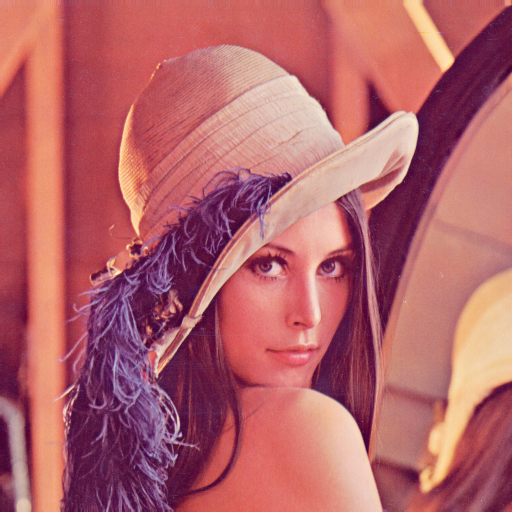
\includegraphics[height=0.8\textheight]{pictures/Lenna.png}
                \end{center} 
            \end{frame}

            \begin{frame}
                \begin{center}
                    \frametitle{Jak zapisać obraz?}
                    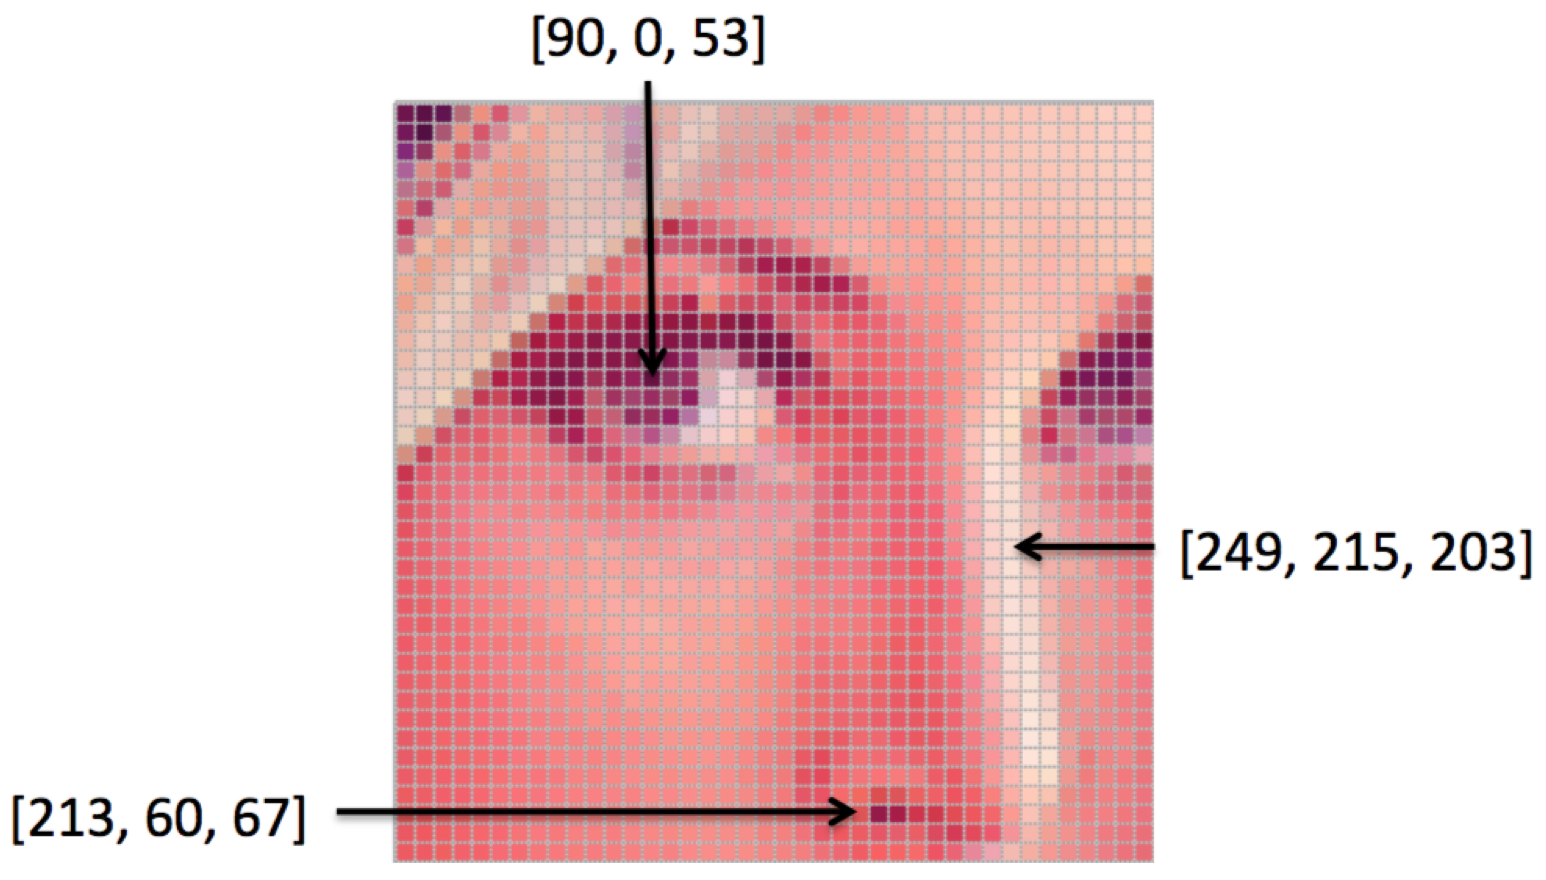
\includegraphics[width=0.8\textwidth]{pictures/colorpixels.png}
                \end{center}
            \end{frame}

            \begin{frame}
                \begin{center}
                    \frametitle{Jak zapisać obraz?}
                    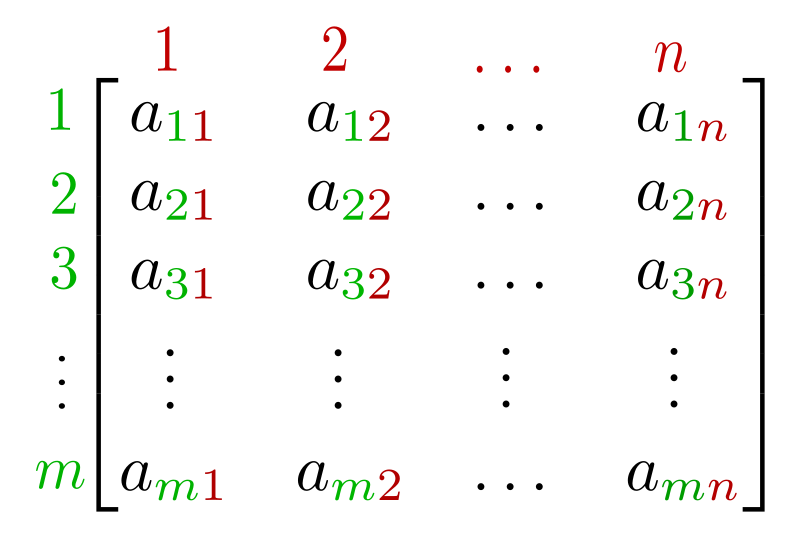
\includegraphics[width=0.8\textwidth]{pictures/matrix.png}
                \end{center}
            \end{frame}
        
        \subsection{Przetwarzanie obrazu. Definicja i zastosowania}

            \begin{frame}
                \frametitle{Czym jest przetwarzanie obrazu}
                Przetwarzanie obrazu (computer vision): dziedzina zajmująca się rozwojem technik pozwalających na odzyskiwanie ze zdjęć trójwymiarowego wyglądu obiektów [A1]
            \end{frame}

            \begin{frame}
                \frametitle{Przetwarzanie obrazu w służbie człowiekowi}
                \begin{itemize}
                    \item diagnostyka medyczna
                    \item Optical Character Recognition i Optical Mark Recognition
                    \item autonomiczne pojazdy
                    \item wspomaganie osób z niepełnosprawnościami
                    \item rozpoznawanie dźwięku
                    \item w dronach - patrolowanie zbiorów, poszukiwania ludzi w pożarach, zawalonych budynkach, itp [A1]
                \end{itemize}
            \end{frame}

            \begin{frame}
                \begin{center}s
                    \frametitle{Co można zrobić z Twoim zdjęciem}
                    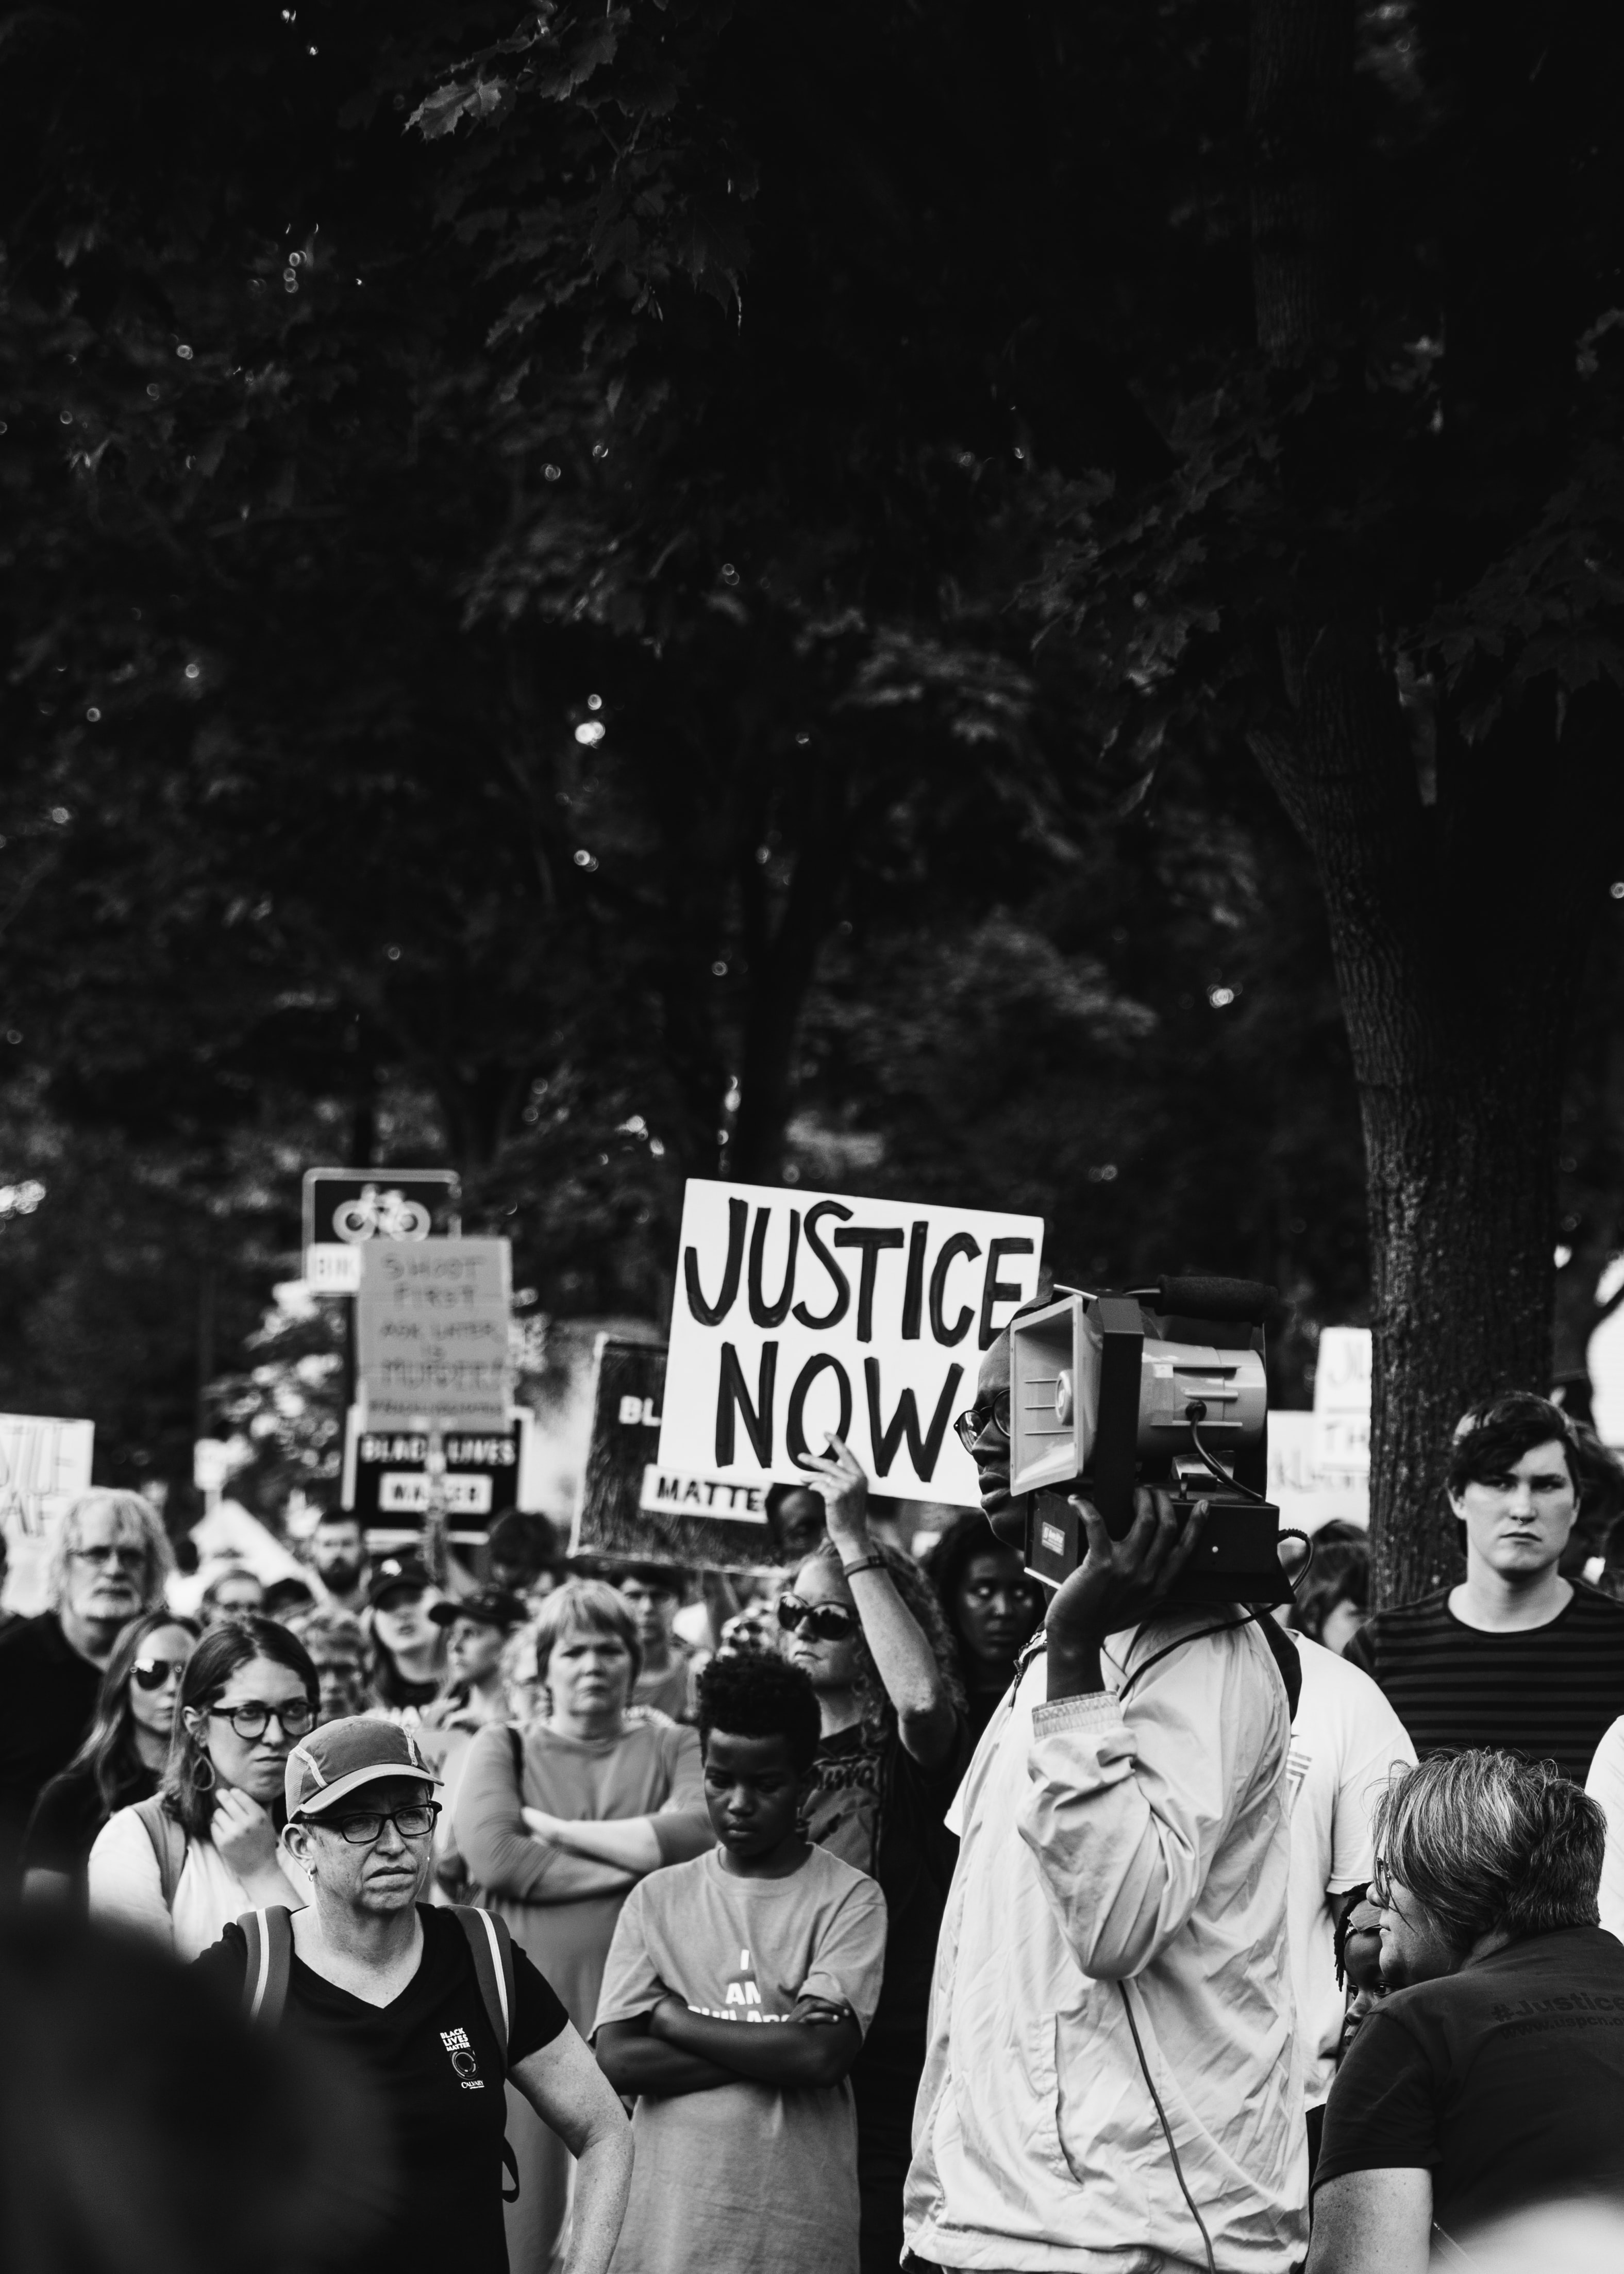
\includegraphics[height=0.8\textheight]{pictures/protest.jpg}
                \end{center}
            \end{frame}

            \begin{frame}
                \begin{center}
                    \frametitle{Co można zrobić z Twoim zdjęciem}
                    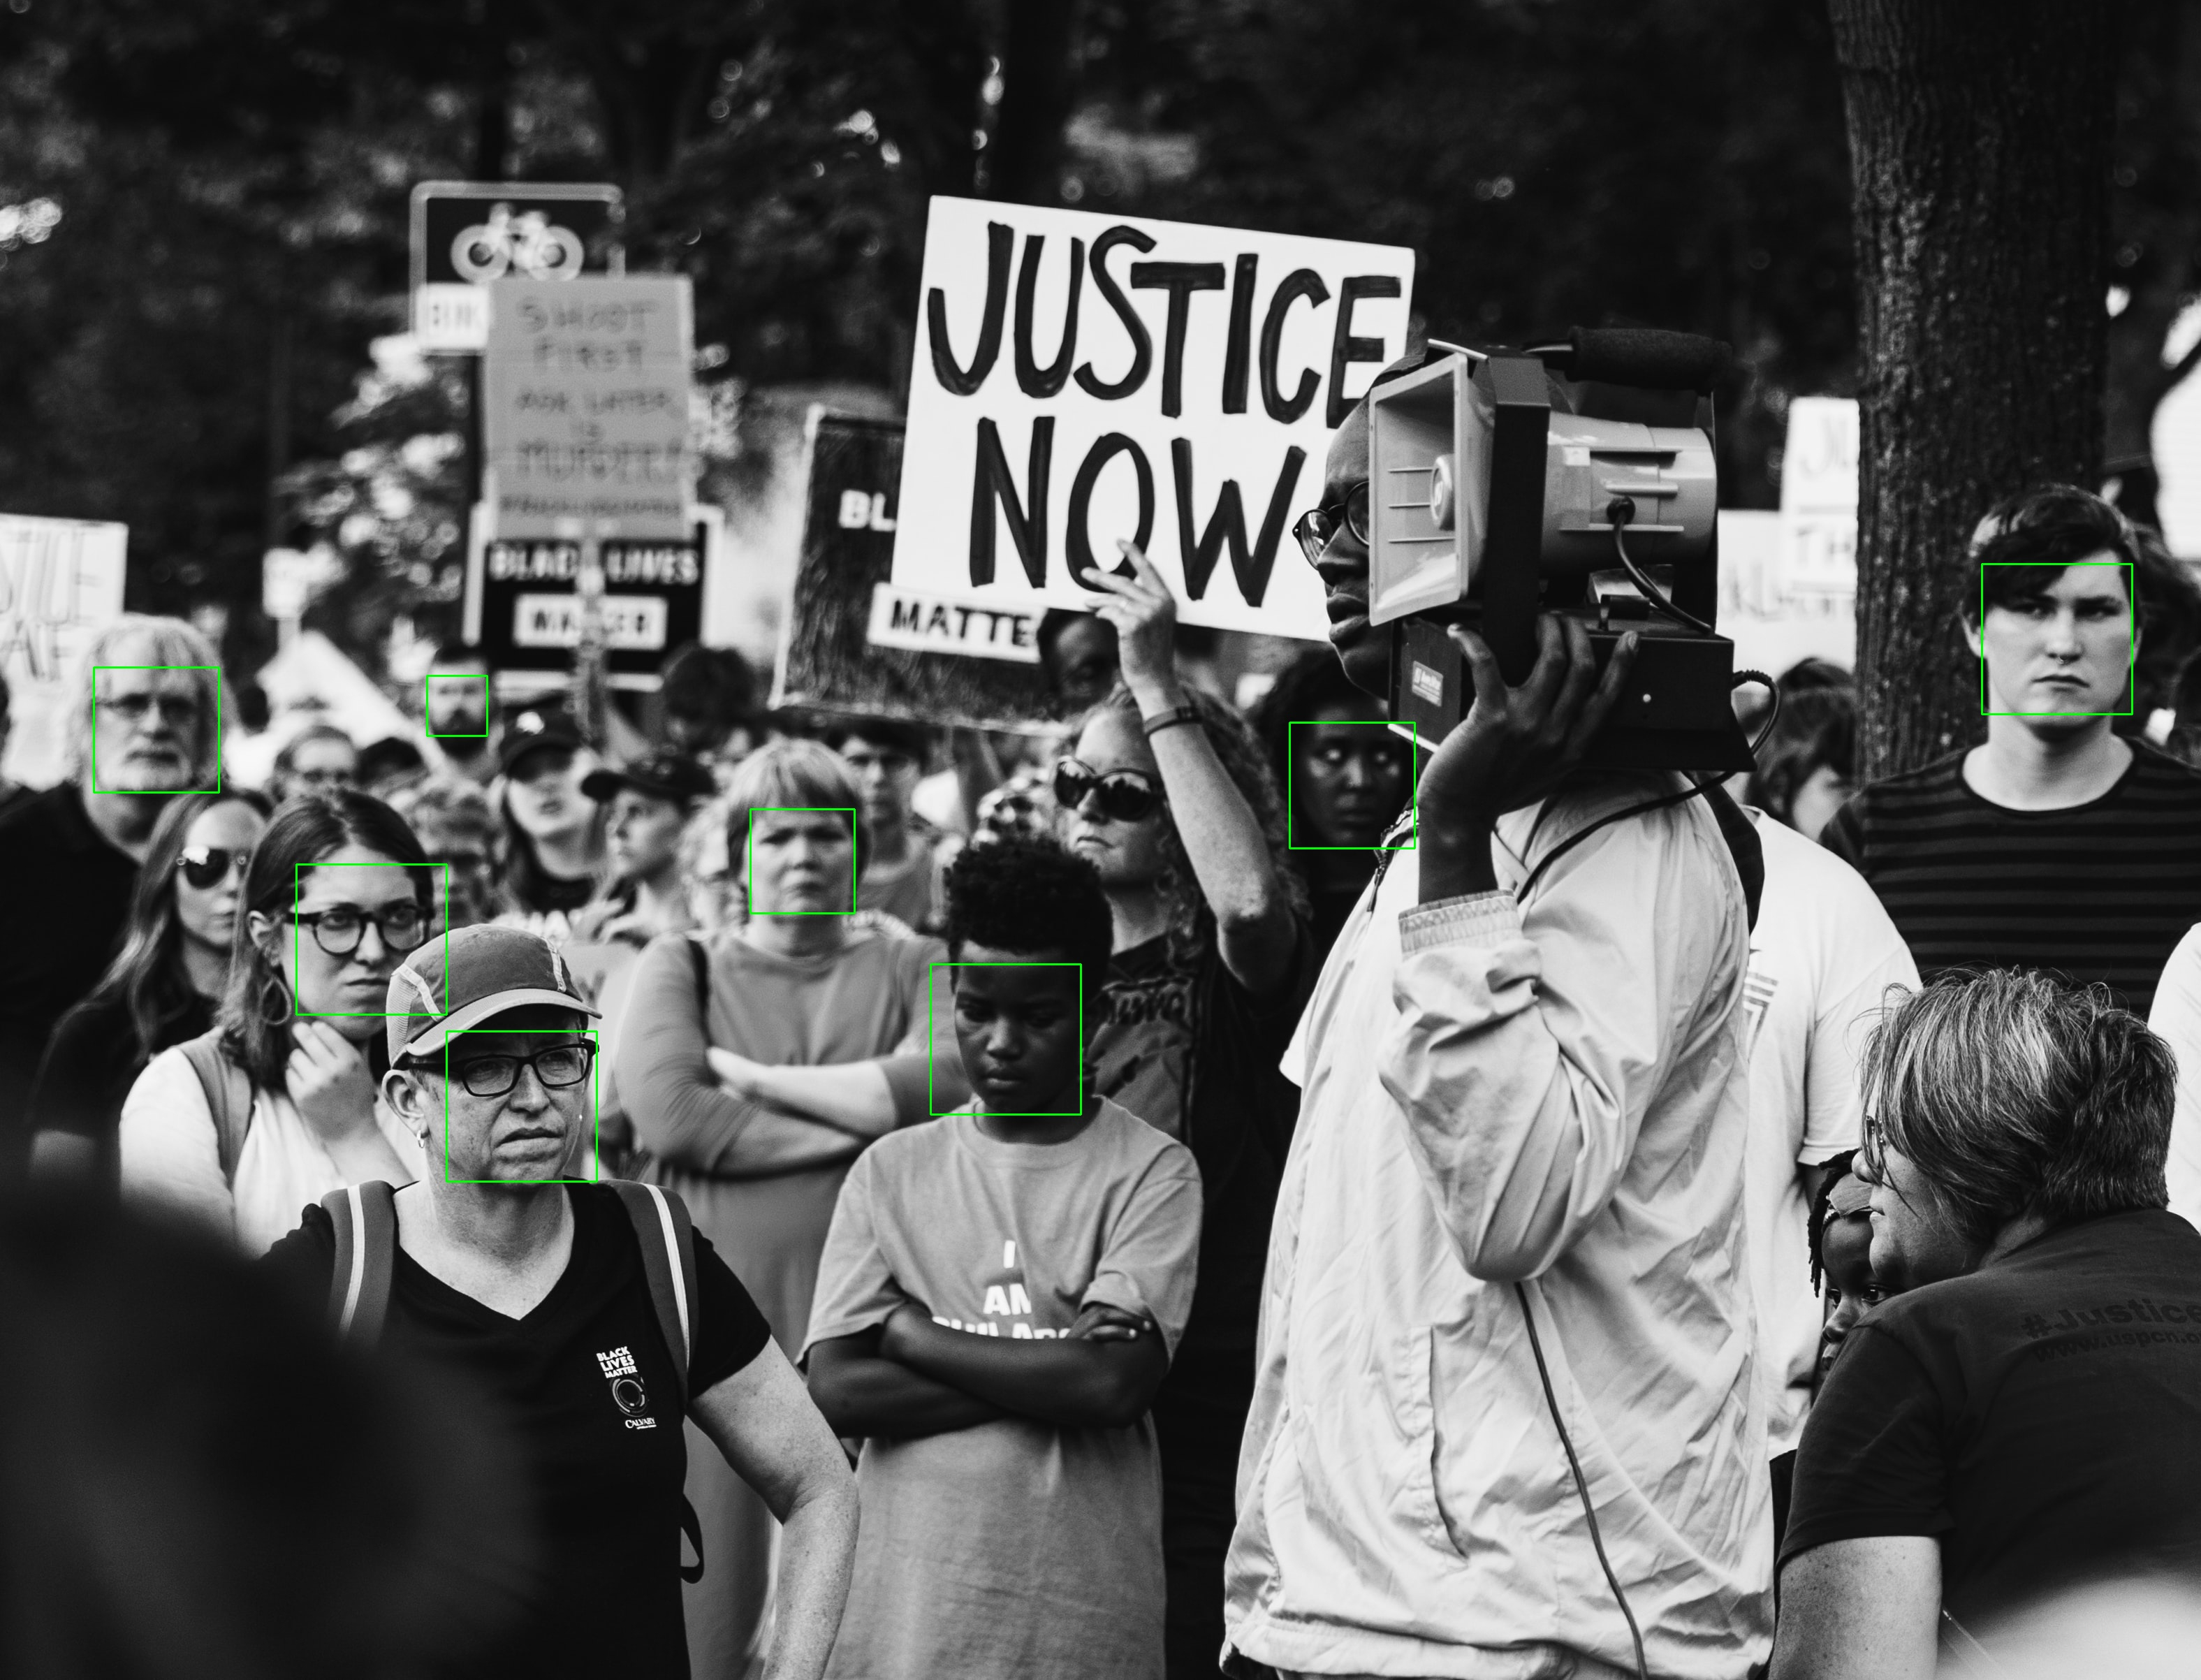
\includegraphics[height=0.8\textheight]{pictures/protest_faces.jpg}
                \end{center}
            \end{frame}

            \begin{frame}
                \begin{center}
                    \frametitle{Co można zrobić z Twoim zdjęciem}
                    \begin{columns}
                        \begin{column}{0.5\textwidth}
                            \begin{center}
                                
\includegraphics[width=0.5\textwidth]{pictures/clearview_ai.png}
                            \end{center}
                        \end{column}
                        \begin{column}{0.5\textwidth}
                            Clearview AI has expanded to at least 26 countries outside the US, engaging national law enforcement agencies, government bodies, and police forces in Australia, Belgium, Brazil, Canada, Denmark, Finland, France, Ireland, India, Italy, Latvia, Lithuania, Malta, the Netherlands, Norway, Portugal, Serbia, Slovenia, Spain, Sweden, Switzerland, and the United Kingdom. [B2]
                        \end{column}
                    \end{columns}
                \end{center}
            \end{frame}

    \section{Sposoby wykrywania obiektów (twarzy) na zdjęciach}
        
        \subsection{Popularne metody}
            \begin{frame}
                \frametitle{Popularne metody}
                \begin{columns}
                    \begin{column}{0.5\textwidth}
                        \begin{itemize}
                            \item Algorytm Viola-Jonesa
                            \item Histogram zorientowanych gradientów
                            \item Głębokie uczenie maszynowe,\\ w szczególności konwolucyjne sieci neuronowe (CNNs)
                        \end{itemize}
                    \end{column}
                    \begin{column}{0.5\textwidth}
                        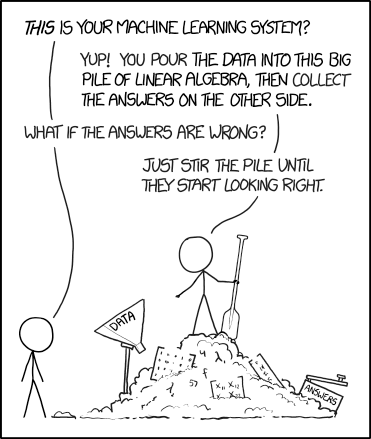
\includegraphics[width=1\textwidth]{pictures/machine_learning.png}
                    \end{column}
                \end{columns}
            \end{frame}

        \subsection{Histogramy zorientowanych gradientów: omówienie}
            \begin{frame}
                \frametitle{Gradient i zorientowane gradienty}
                \begin{columns}
                    \begin{column}{0.5\textwidth}
                        \begin{center}
                            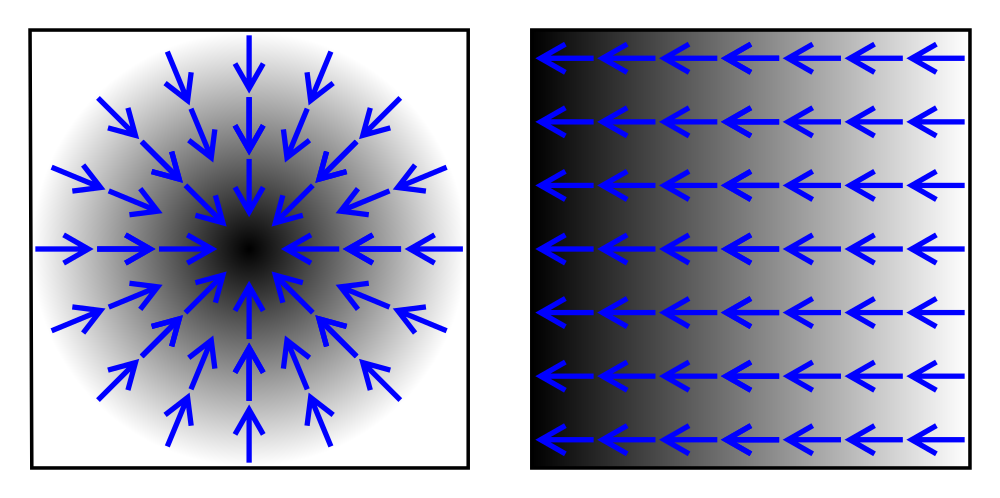
\includegraphics[width=1\textwidth]{pictures/gradient.png}
                        \end{center}
                            Wielkość wektora gradientu: $\sqrt{\left( f^{2}_{x}+f^{2}_{y}\right)}$.
                            \newline
                            \newline
                            Kąt wektora gradientu: $\arctan{\frac{f_{y}}{f_{x}}}$.
                    \end{column}
                    \begin{column}{0.5\textwidth}
                        \begin{center}
                            
\includegraphics[width=0.5\textwidth]{pictures/circle.png}
                            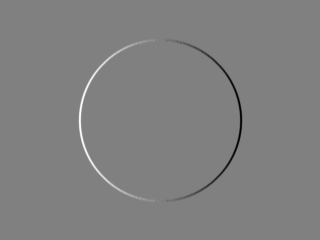
\includegraphics[width=0.5\textwidth]{pictures/gradient_x.png}
                            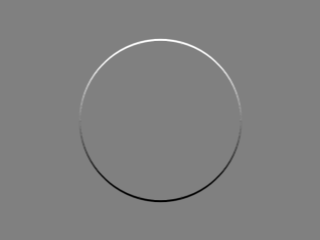
\includegraphics[width=0.5\textwidth]{pictures/gradient_y.png}
                        \end{center}
                    \end{column}
                \end{columns}
            \end{frame}

            \begin{frame}
                \frametitle{Zorientowane gradienty: przykład}
                \begin{columns}
                    \begin{column}{0.5\textwidth}
                        \begin{center}
                            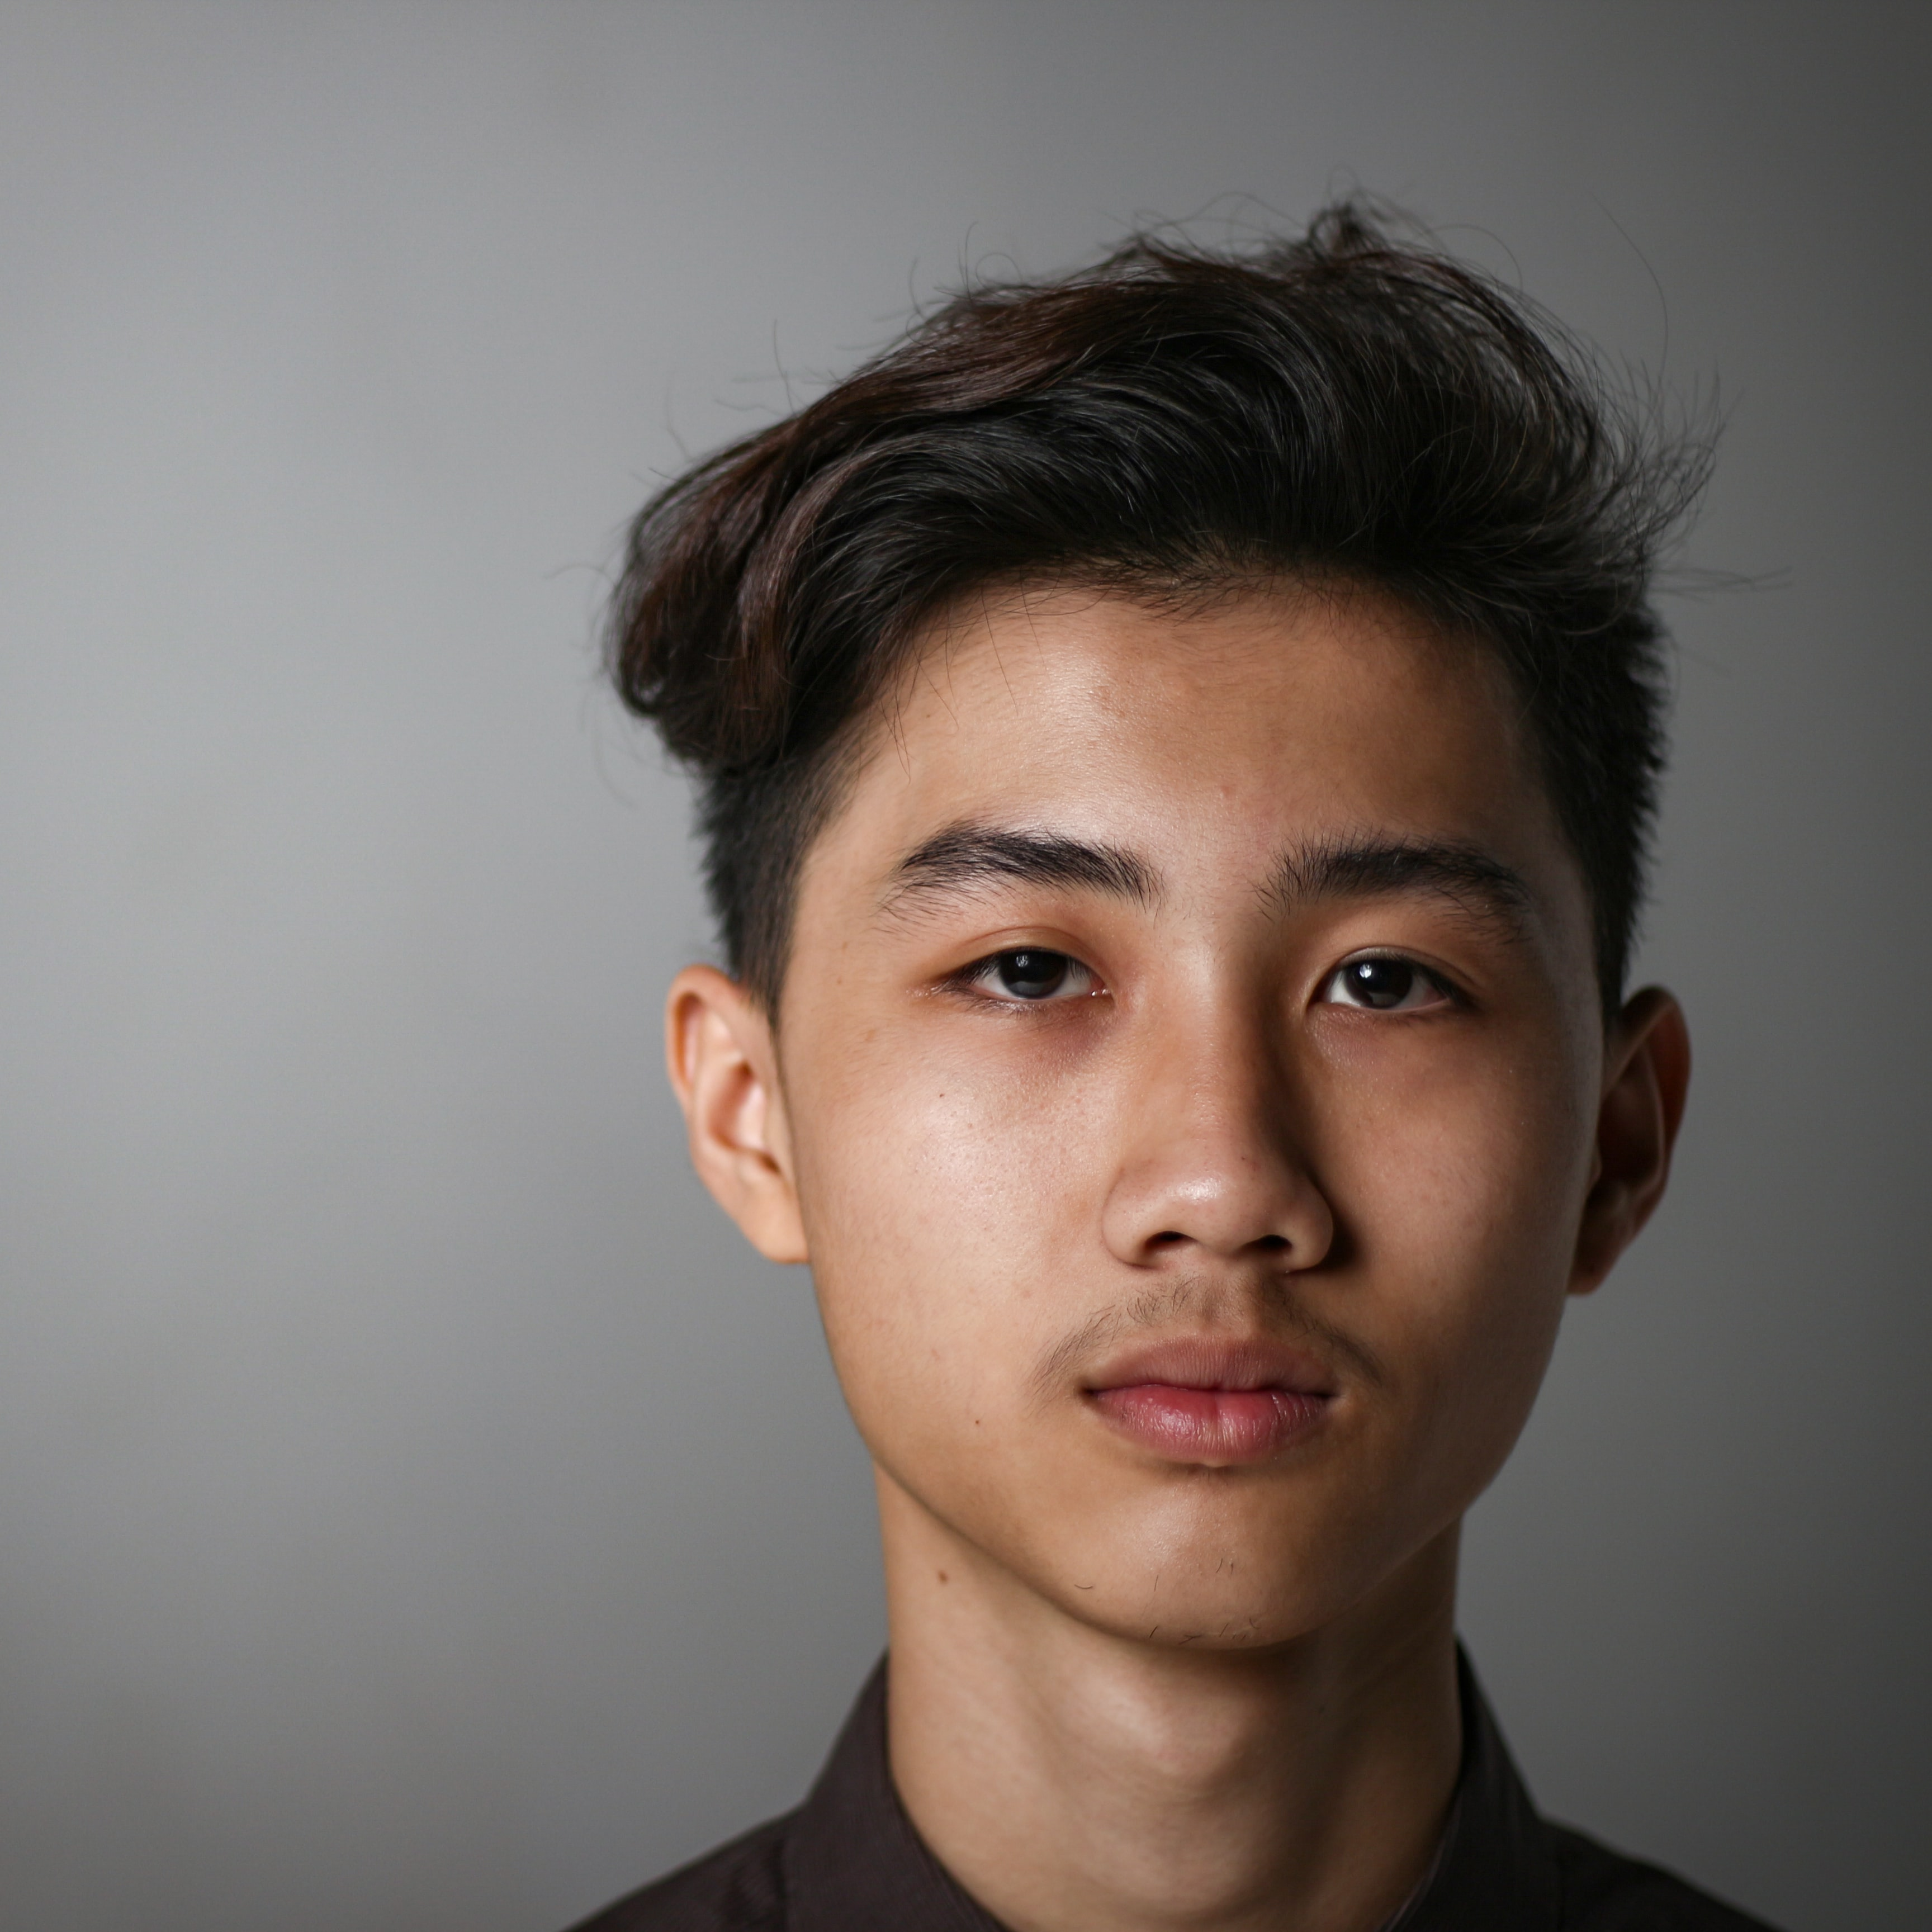
\includegraphics[width=0.8\textwidth]{pictures/face_unsplash}
                        \end{center}
                    \end{column}
                    \begin{column}{0.5\textwidth}
                            $\begin{pmatrix}
                                128 & 136 & 119\\
                                142 & 132 & 147\\
                                136 & 148 & 161
                            \end{pmatrix}$
                            \newline
                            \newline
                            \newline
                            $f_{x}=147-142$
                            \newline
                            $f_{y}=148-136$
                            \newline
                            \newline
                            Wielkość wektora gradientu: $\sqrt{\left( 5^{2}+12^{2}\right)} = 13$.
                            \newline
                            \newline
                            Kąt wektora gradientu: $\arctan{5/12} \approx 23^\circ$.
                    \end{column}
                \end{columns}
            \end{frame}

            \begin{frame}
                \frametitle{Zorientowane gradienty: przykład}
                \begin{columns}
                    \begin{column}{0.5\textwidth}
                        \begin{center}
                            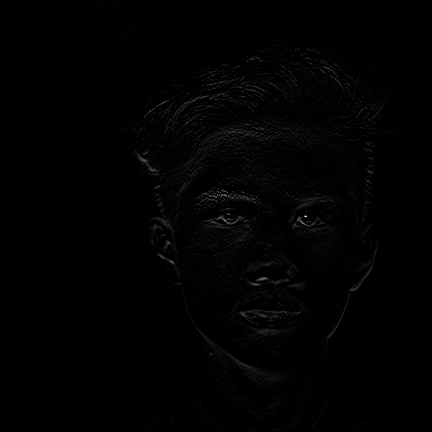
\includegraphics[width=0.6\textwidth]{pictures/x_sobel}
                            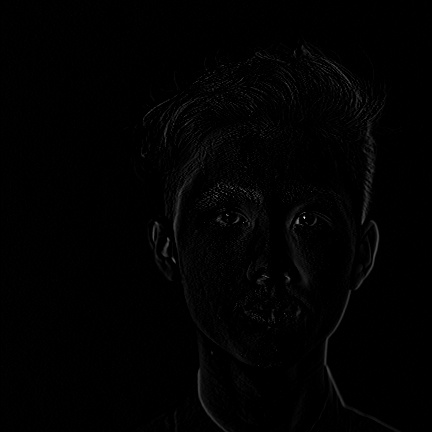
\includegraphics[width=0.6\textwidth]{pictures/y_sobel}
                        \end{center}
                    \end{column}
                    \begin{column}{0.5\textwidth}
                        \begin{center}
                            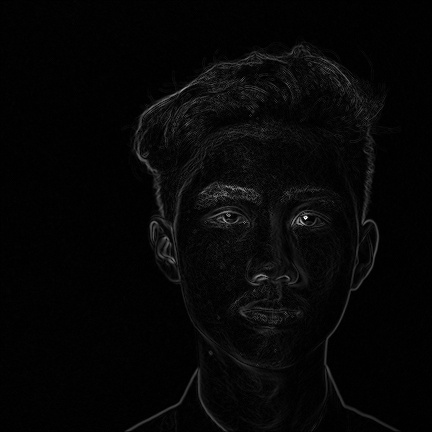
\includegraphics[width=0.6\textwidth]{pictures/magnitude}
                            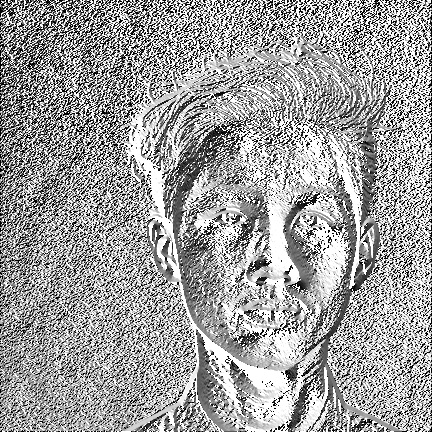
\includegraphics[width=0.6\textwidth]{pictures/angle.jpg}
                        \end{center}
                    \end{column}
                \end{columns}
            \end{frame}

            \begin{frame}
                \frametitle{Histogram zorientowanych gradientów}
                        Wielkości wektorów: $\begin{pmatrix}
                            25 & 18\\
                            15 & 10
                        \end{pmatrix}$, 
                        kąty wektorów: $\begin{pmatrix}
                            47 & 172\\
                            42 & 50
                        \end{pmatrix}$
                        \newline
                        \newline
                        \begin{center}
                            \begin{tabular}{ |c|c|c|c|c|c|c|c|c| }
                                \hline
                                    0 & 20 & 40 & 60 & 80 & 100 & 120 & 140 & 160\\
                                    \hline
                                    0 & 0 & 0 & 0 & 0 & 0 & 0 & 0 & 0\\
                                    0 & 0 & 25 & 0 & 0 & 0 & 0 & 0 & 0\\
                                    18 & 0 & 25 & 0 & 0 & 0 & 0 & 0 & 0\\
                                    18 & 0 & 40 & 0 & 0 & 0 & 0 & 0 & 0\\
                                    18 & 0 & 45 & 5 & 0 & 0 & 0 & 0 & 0\\
                                \hline
                            \end{tabular}
                        \end{center}
                        Tym sposobem z 8x8x3 => 8x8x2 => 9 wartości opisujących podobraz.
            \end{frame}

            \begin{frame}
                \frametitle{Histogram zorientowanych gradientów: przykład}
                \begin{center}
                    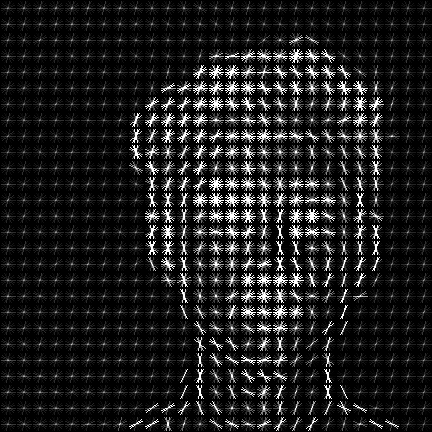
\includegraphics[height=0.8\textheight]{pictures/hog_exposed.png}
                \end{center}
            \end{frame}

    \section{Atak: jak zdezorientować gradienty?}

            \begin{frame}
                \frametitle{Czasami gradienty same się dezorientują}
                \begin{center}
                    \begin{figure}
                        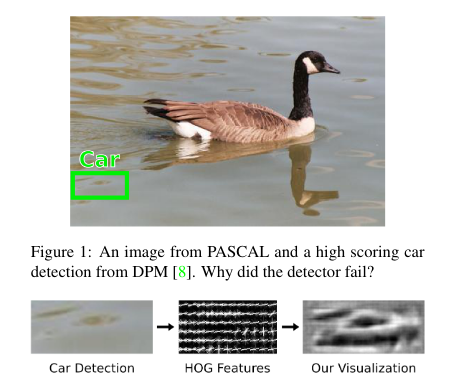
\includegraphics[height=0.75\textheight]{pictures/vondrick_duck.png}
                        \caption{If it looks like a car and it honks like a car... [A3]}
                    \end{figure}
                \end{center}
            \end{frame}

            \begin{frame}
                \frametitle{Twarz klasyfikatora}
                \begin{center}
                    \begin{figure}
                        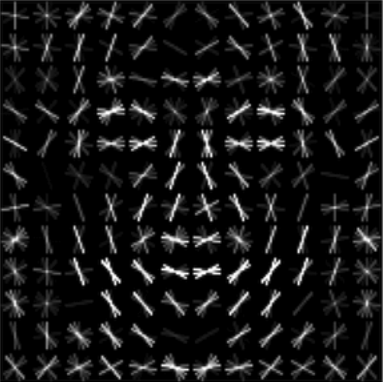
\includegraphics[height=0.75\textheight]{pictures/hog.png}
                        \caption{HOG: wizualizacja 'twarzy człowieka' z biblioteki dlib [C2]}
                    \end{figure}
                \end{center}
            \end{frame}

            \begin{frame}
                \frametitle{Rozpoznawanie twarzy z biblioteką dlib}
                \begin{columns}
                    \begin{column}{0.5\textwidth}
                        \begin{center}
                            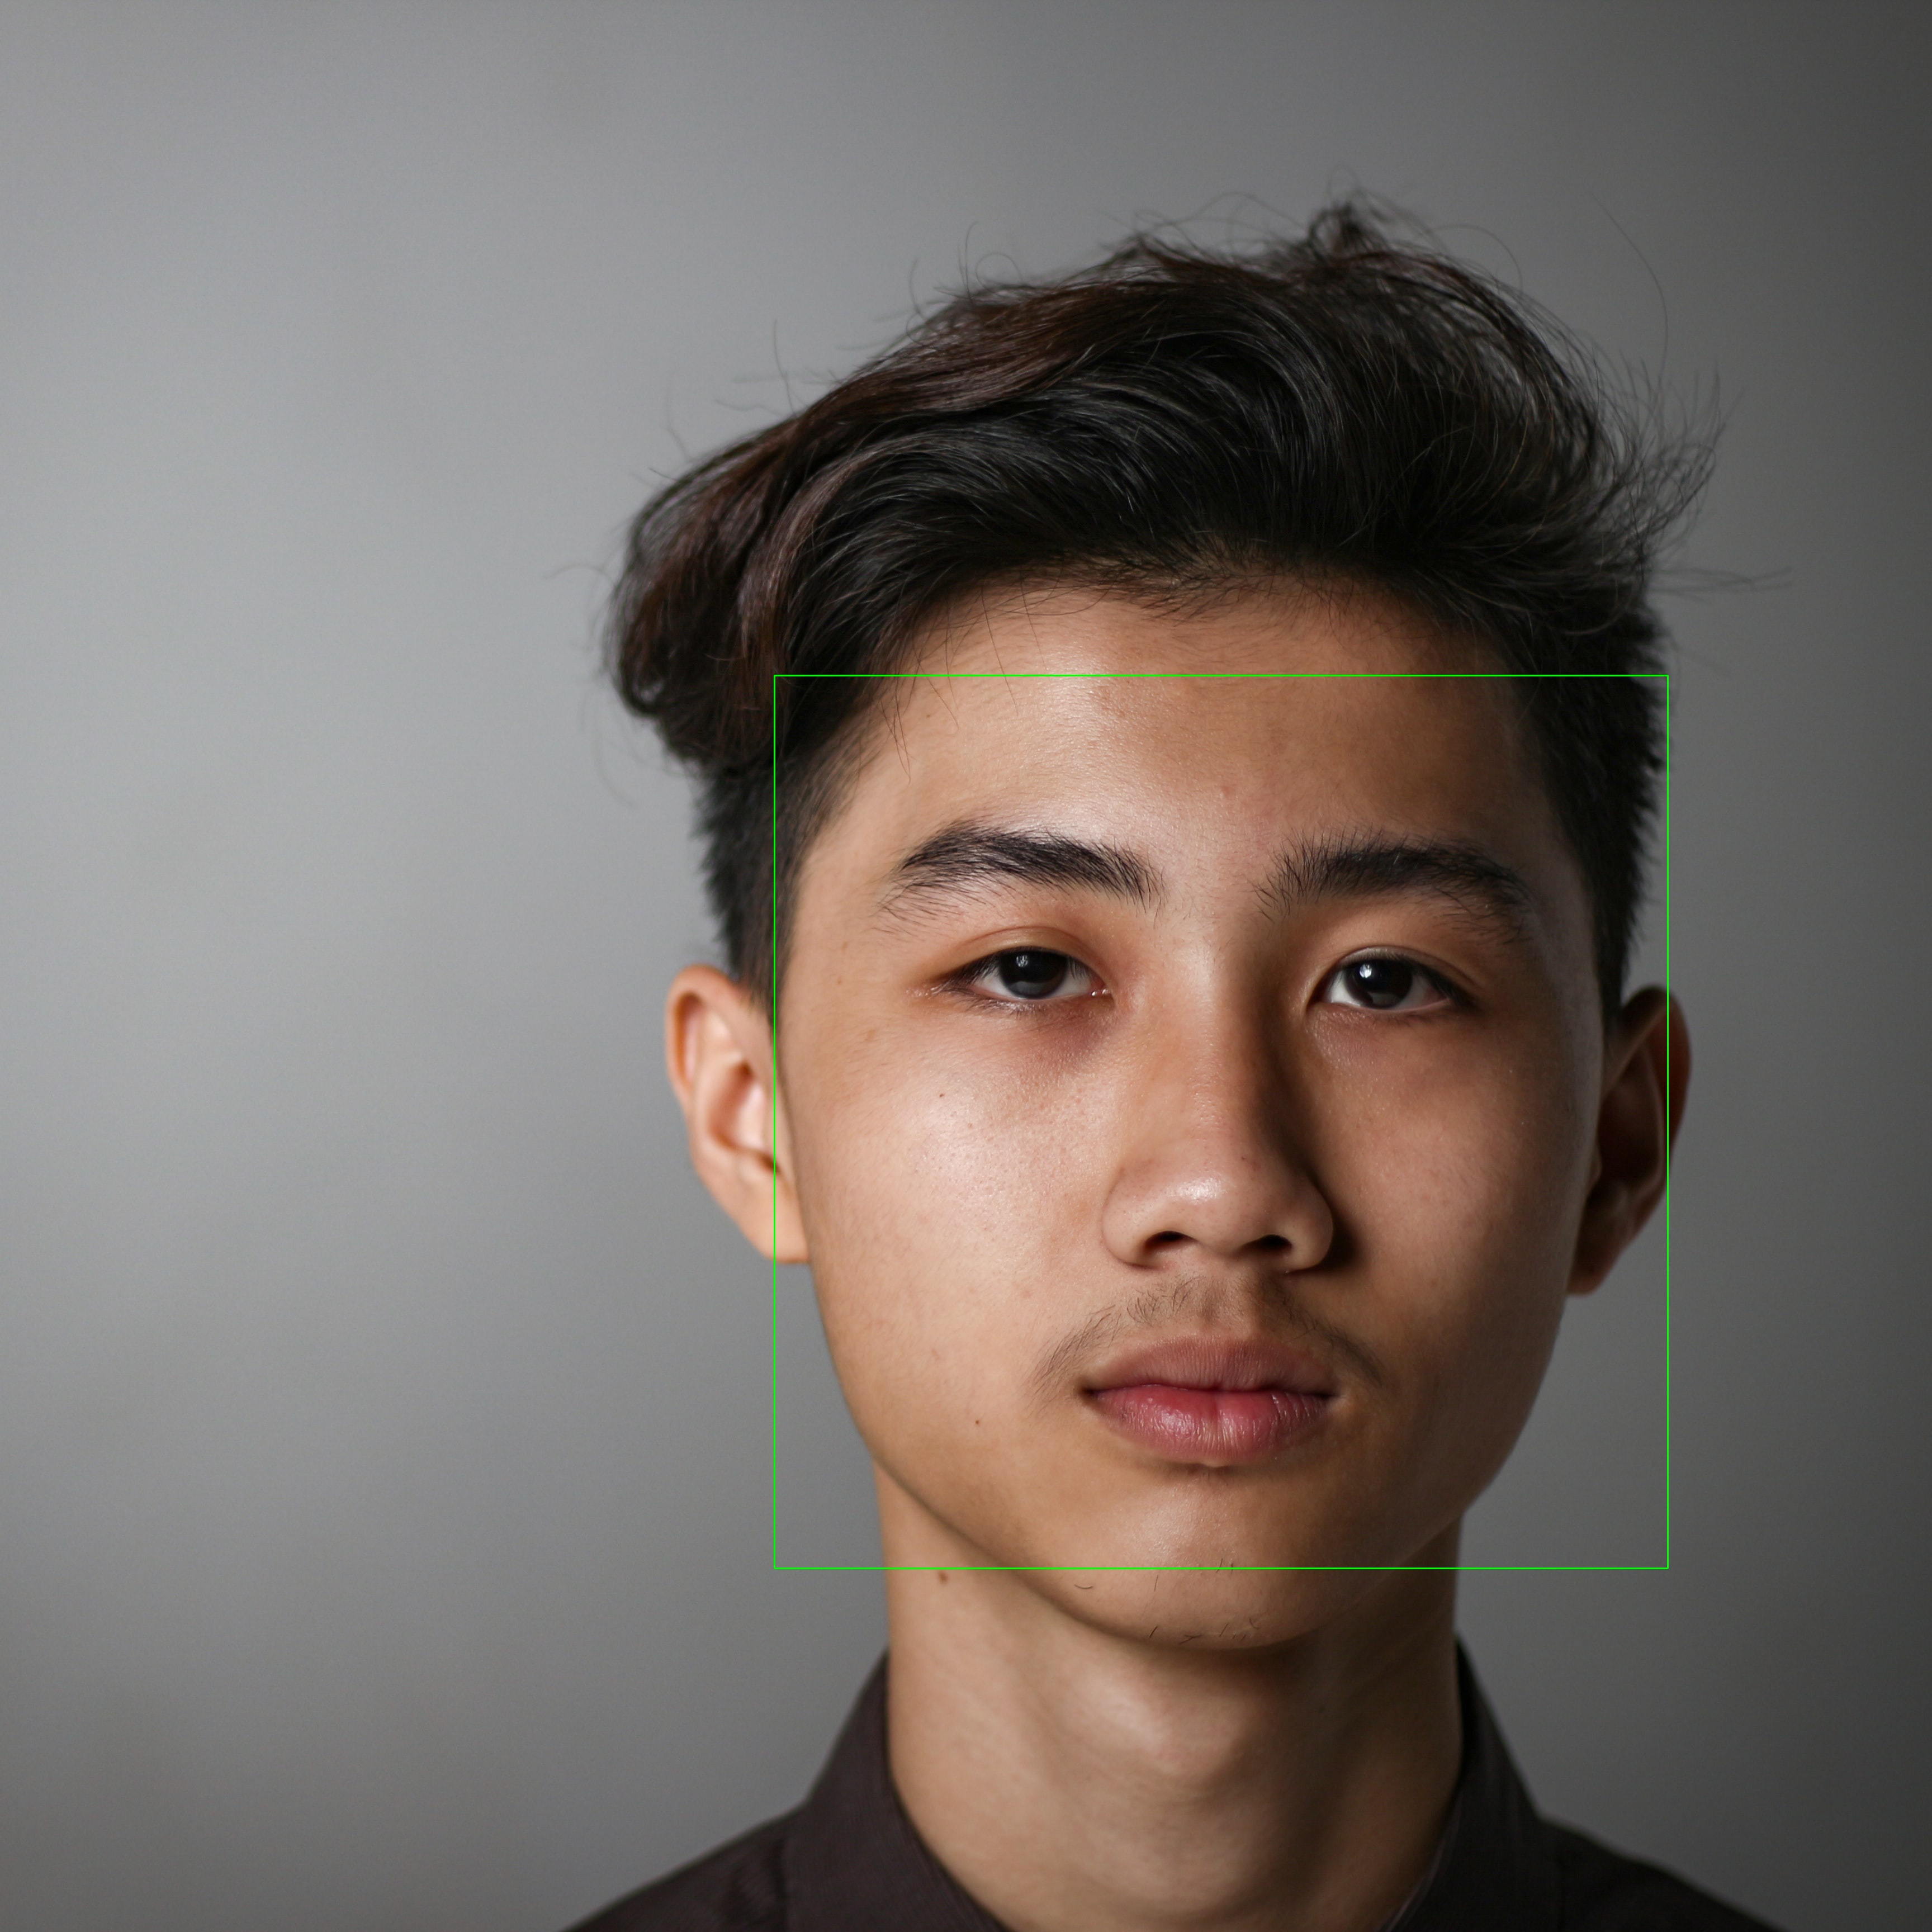
\includegraphics[width=0.9\textwidth]{pictures/face_detected}
                        \end{center}
                    \end{column}
                    \begin{column}{0.5\textwidth}
                        \begin{center}
                            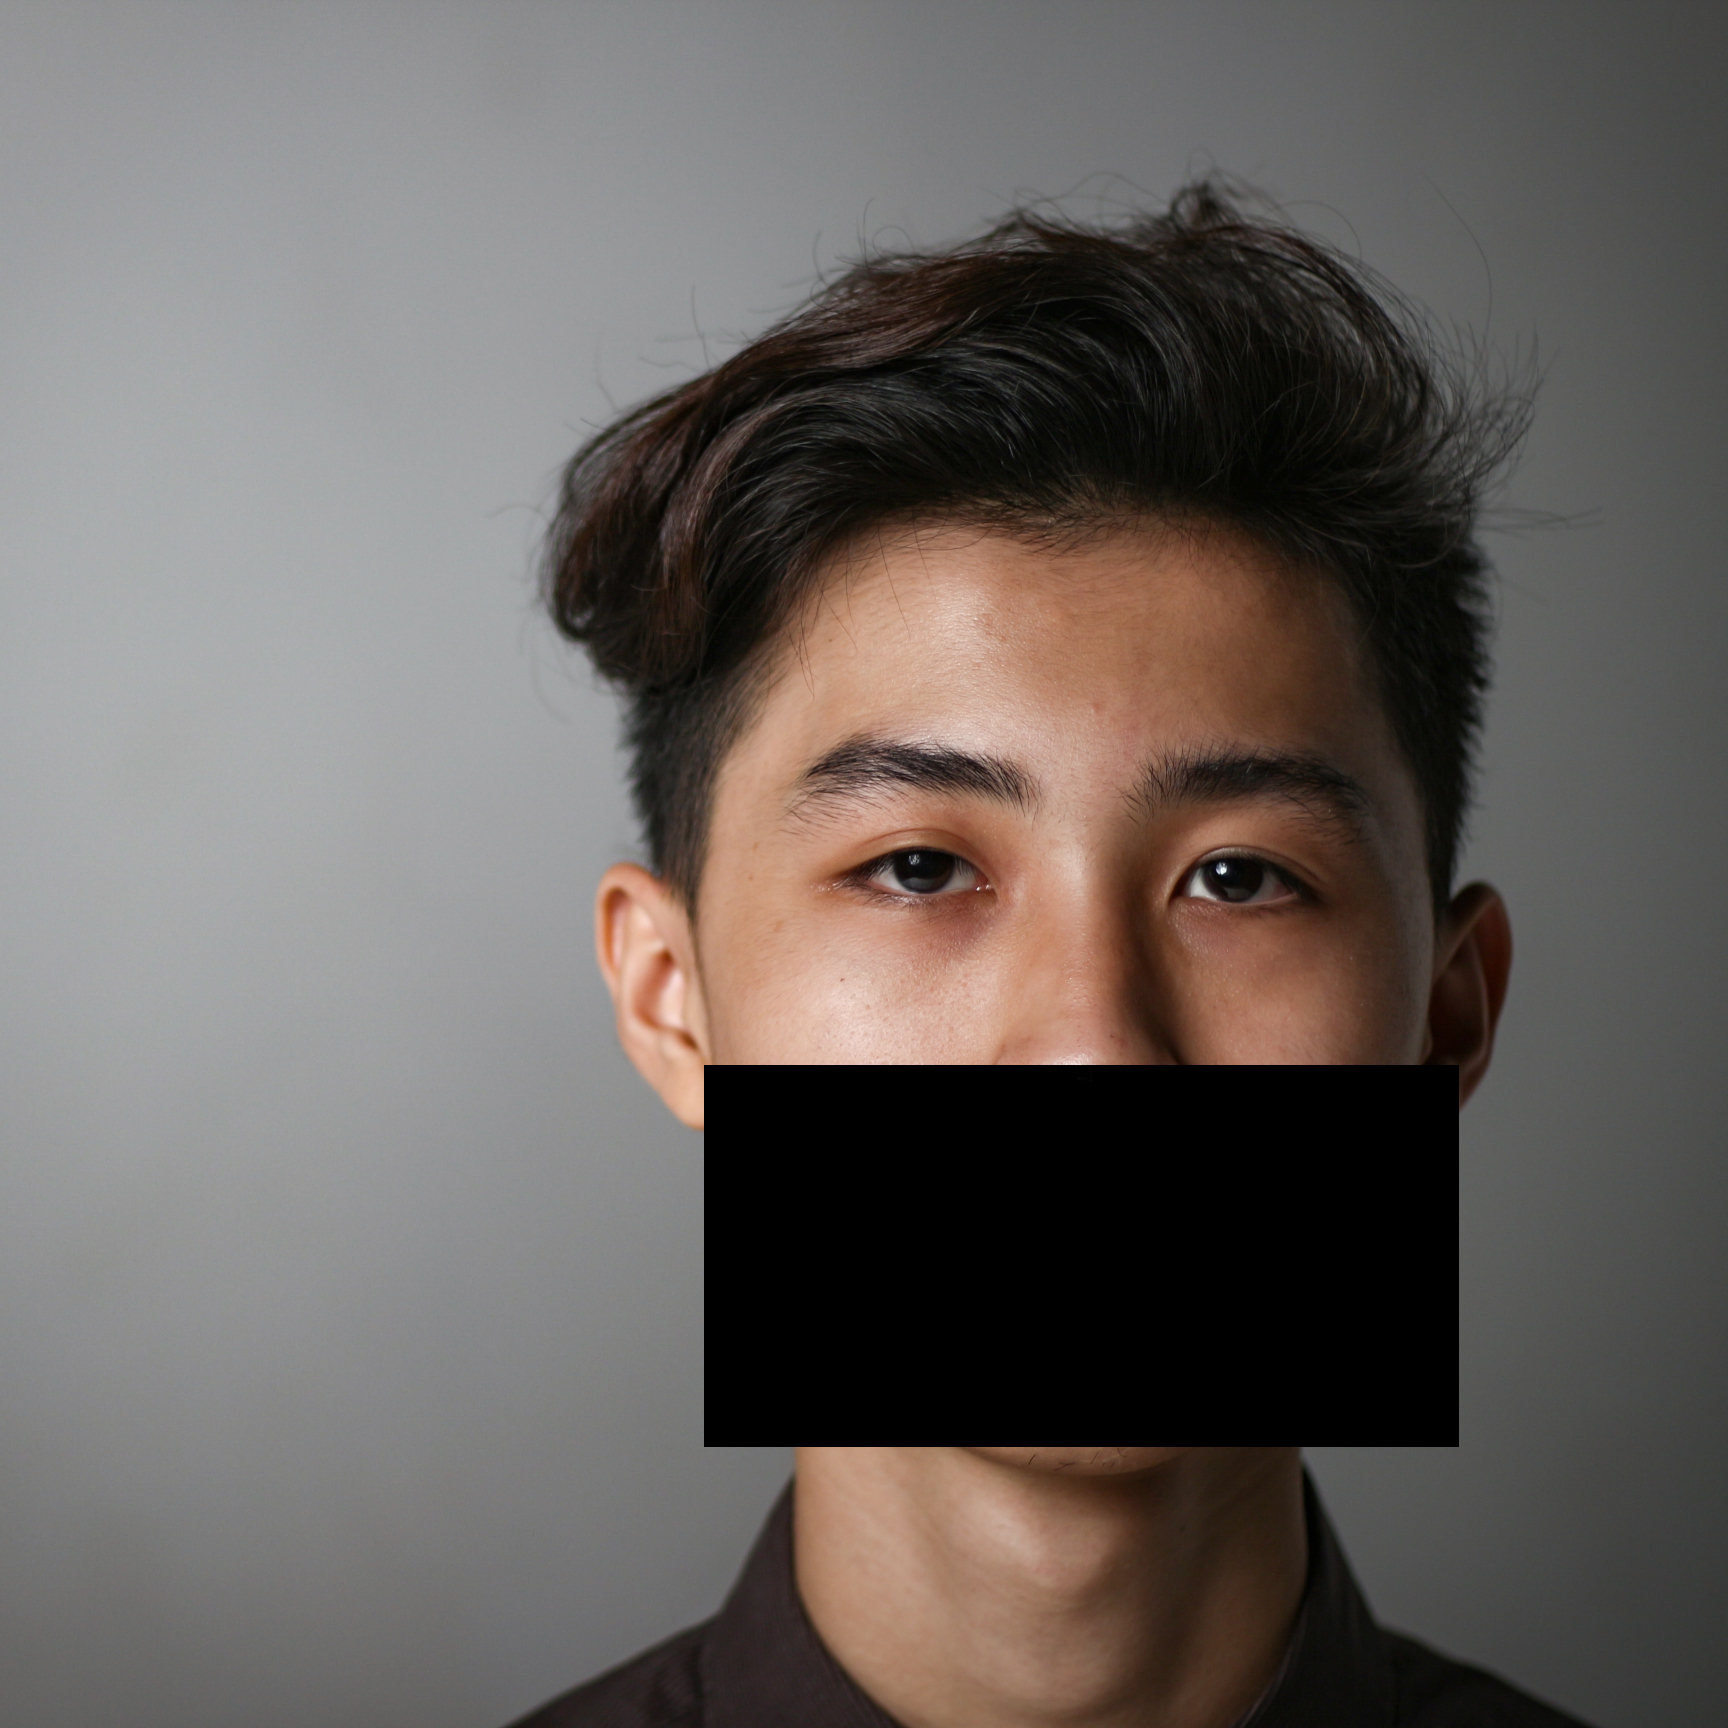
\includegraphics[width=0.9\textwidth]{pictures/face_unsplash_mask}
                        \end{center}
                    \end{column}
                \end{columns}
            \end{frame}

            \begin{frame}
                \frametitle{Rozpoznawanie twarzy z biblioteką dlib}
                \begin{columns}
                    \begin{column}{0.5\textwidth}
                        \begin{center}
                            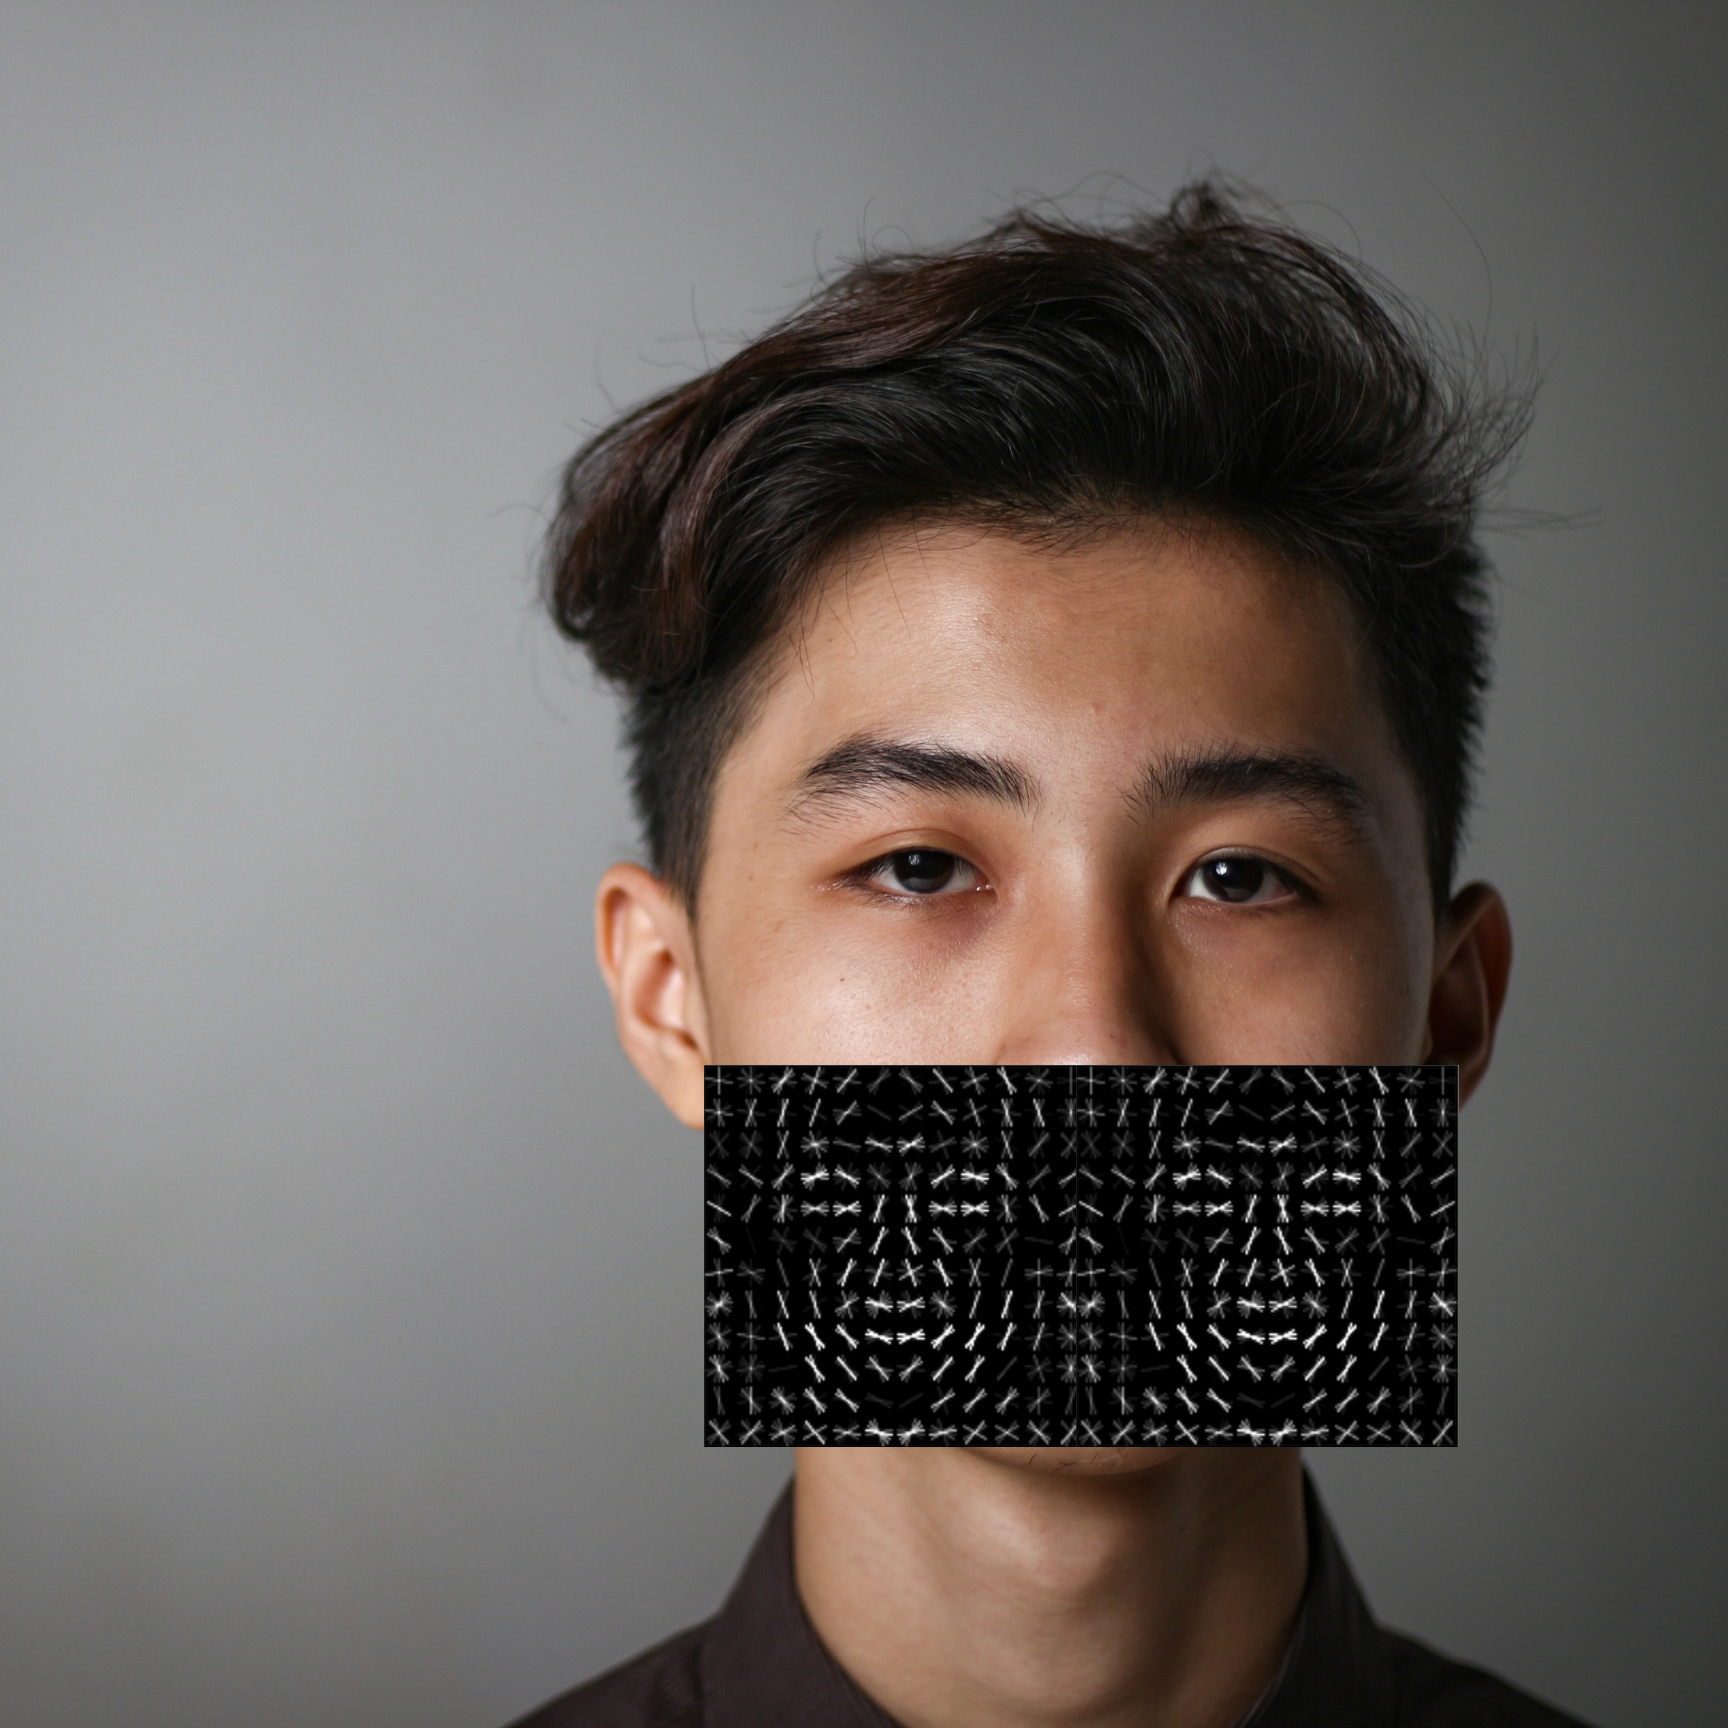
\includegraphics[width=0.9\textwidth]{pictures/face_unsplash_two_hogs}
                        \end{center}
                    \end{column}
                    \begin{column}{0.5\textwidth}
                        \begin{center}
                            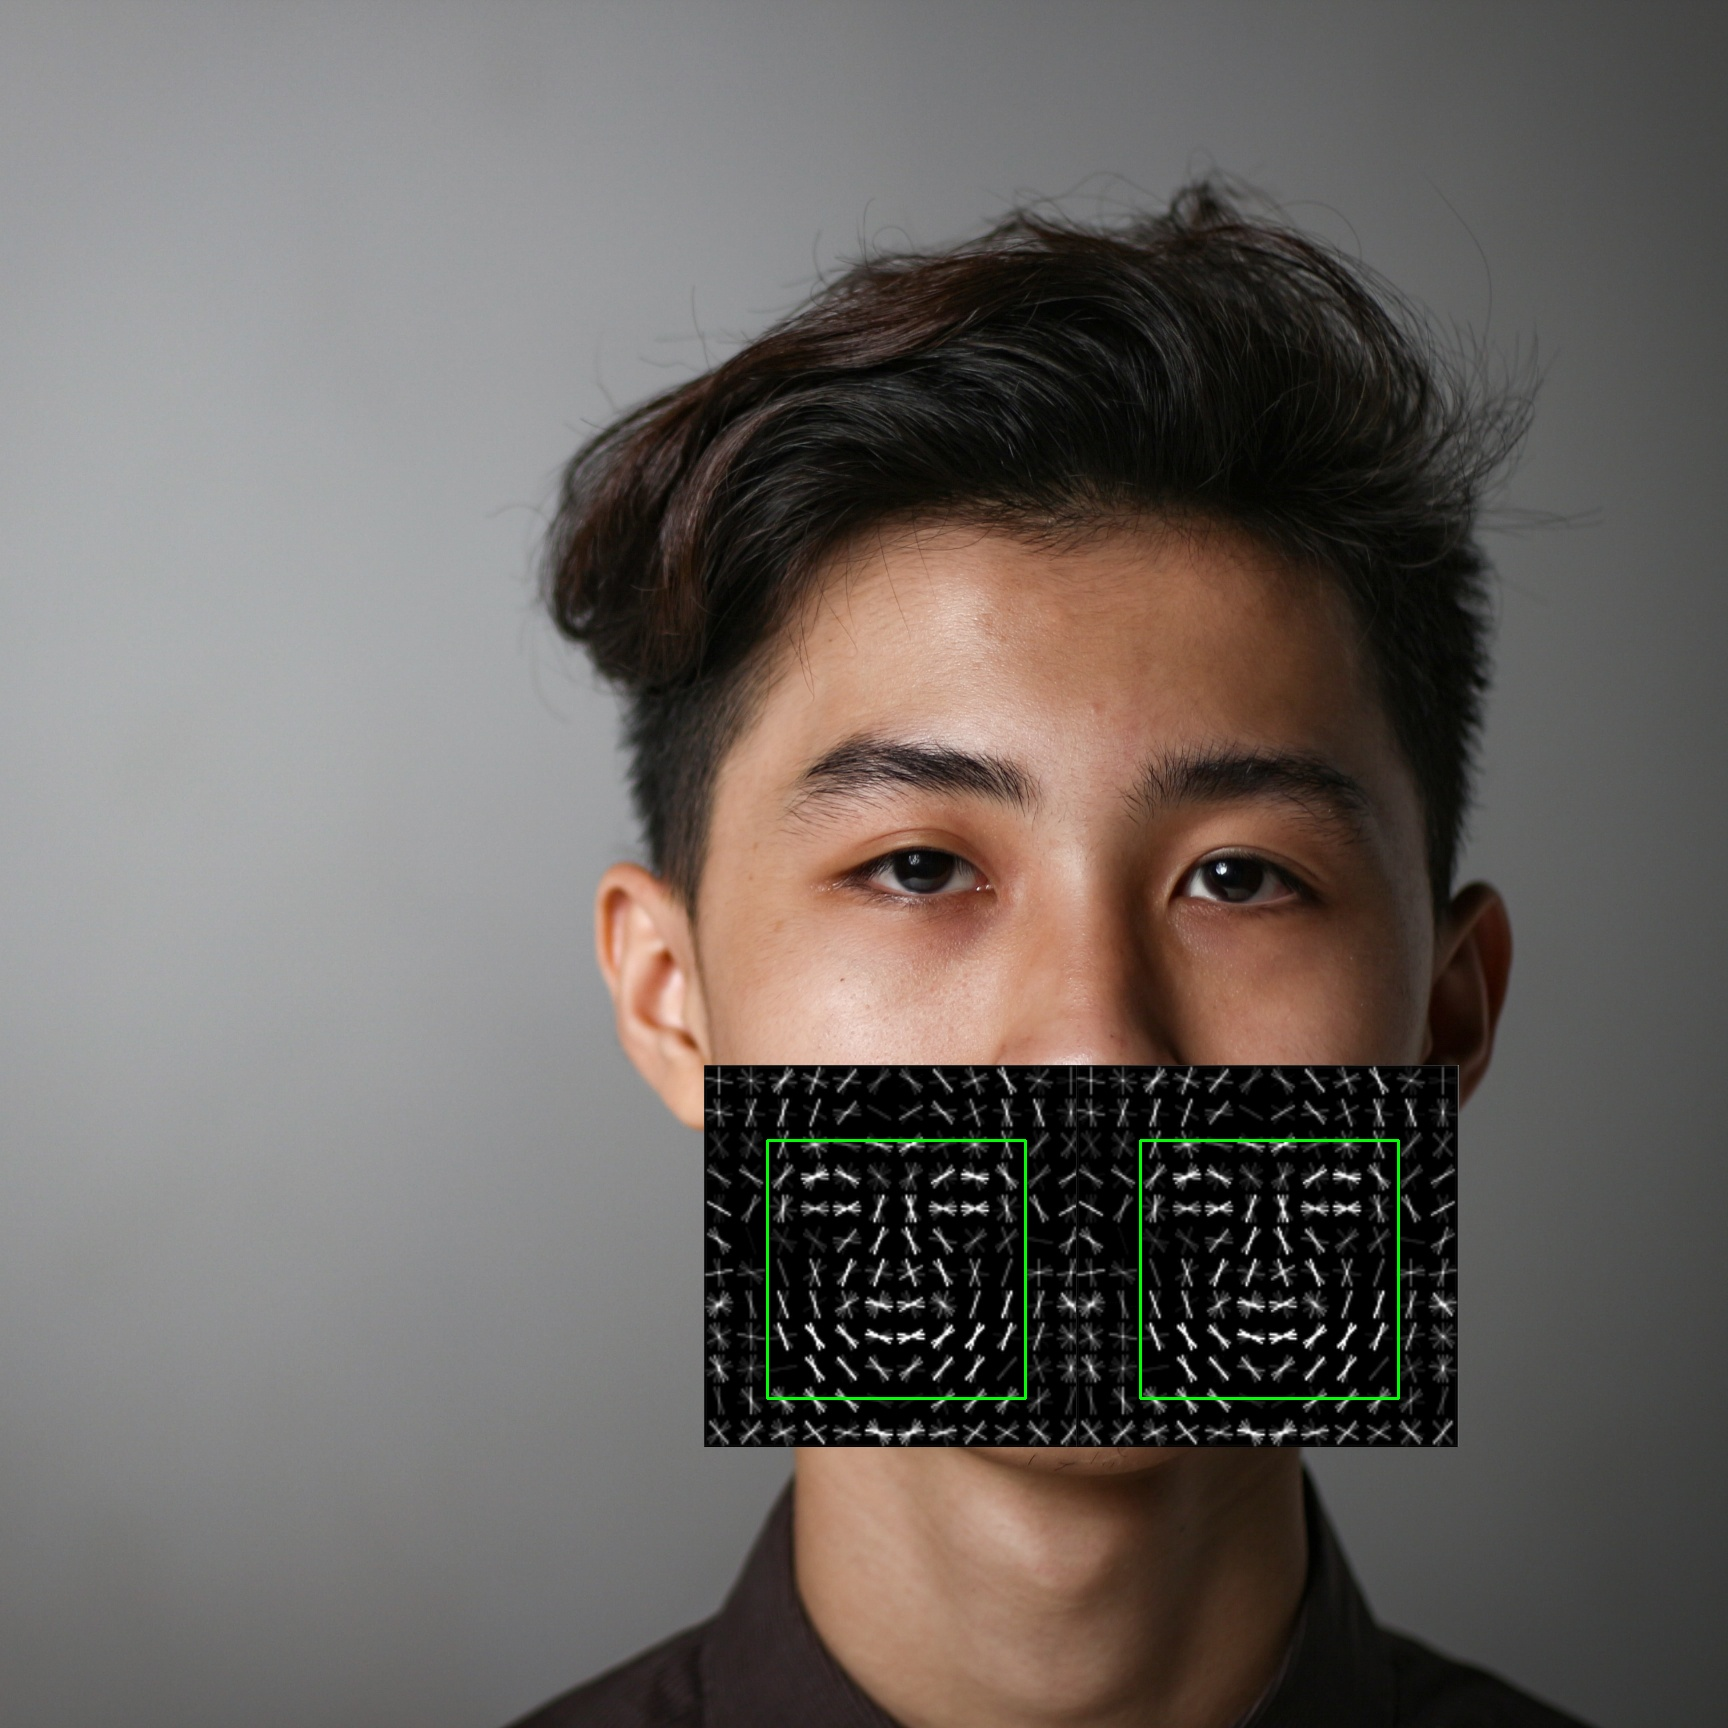
\includegraphics[width=0.9\textwidth]{pictures/face_unsplash_two_hogs_detected}
                        \end{center}
                    \end{column}
                \end{columns}
            \end{frame}

            \begin{frame}
                \frametitle{Zastosowanie w praktyce}
                \begin{center}
                    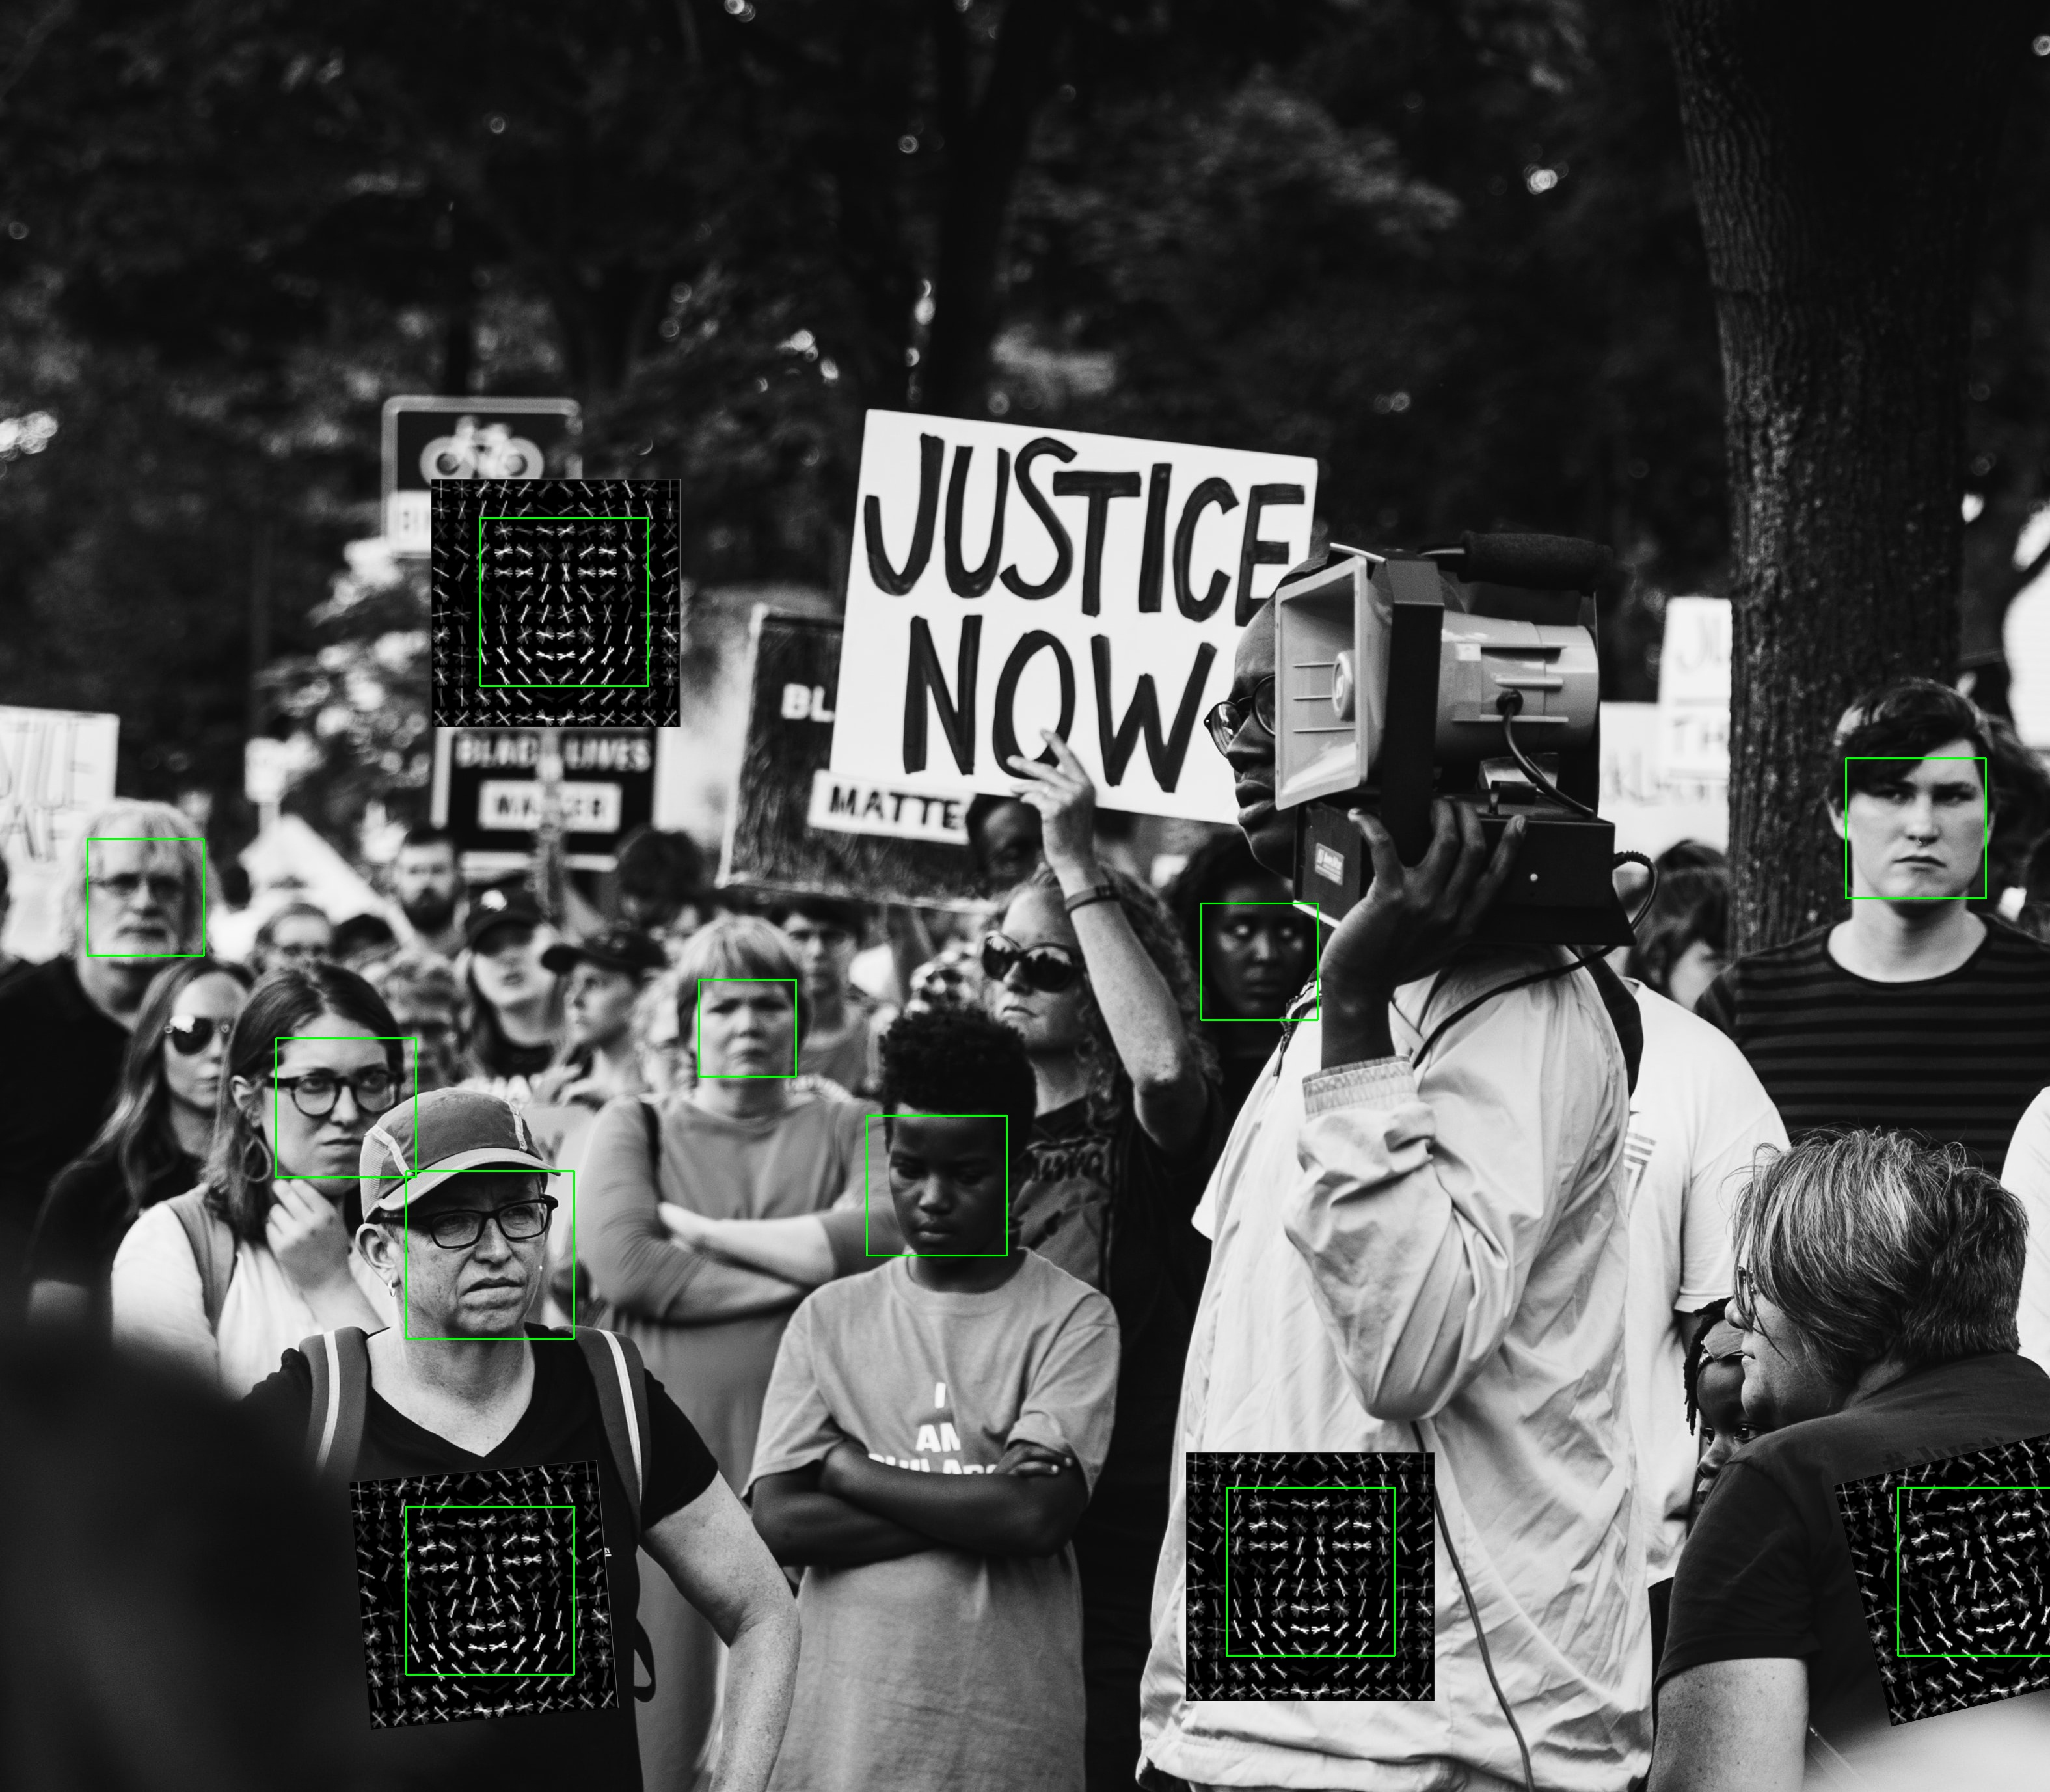
\includegraphics[height=0.8\textheight]{pictures/protest_faces_hogs}
                \end{center}
            \end{frame}

    \section{Podsumowanie}
        \subsection{Wnioski}
            \begin{frame}
                \frametitle{Wnioski}
                \begin{itemize}
                    \item HOG jest dość starą (2005) metodą wykrywania obiektów na zdjęciach, ale jest jednocześnie bardzo łatwy w implementacji (OpenCV + dlib)
                    \item Bez względu na użytą metodę wykrywania, systemy są podatne na ataki i można to wykorzystać w różnych celach:
                        \begin{itemize}
                            \item oszukiwanie systemów wykrywania twarzy [A6, A7]
                            \item modyfikowanie znaków drogowych w celu oszukania maszyn [A5, B3]
                            \item podrabianie podpisów tradycyjnych weryfikowanych elektronicznie [A4]
                        \end{itemize}
                    \item Wszystkie Wasze zdjęcia, które postujecie w mediach społecznościowych są publiczne i zostaną użyte bez Waszej wiedzy i zgody do wytrenowania jakichś modeli
                \end{itemize}
            \end{frame}

        \subsection{Źródła}
            \begin{frame}[shrink=15]
                \frametitle{Źródła naukowe (A)}
                \begin{enumerate}
                    \item Szeliski, R. Computer Vision: Algorithms and Applications. Springer: 2010.
                    \item Dalal, N., Triggs, B. Histogram of Oriented Gradients for Human Detection. [In proceedings] IEEE Computer Society Conference on Computer Vision and Pattern Recognition: 2005.
                    \item Vondrick C. et al. HOGgles: Visualizing Object Detection Features. [In proceedings] IEEE International Conference on Computer Vision: 2013.
                    \item Hafemann, L., Sabourin, R. "Characterizing and evaluating adversarial examples for Offline Handwritten Signature Verification.
                        \url{https://arxiv.org/pdf/1901.03398.pdf}
                    \item Eykholt, K. et al. Robust Physical-World Attacks on Deep Learning Visual Classification. [In proceedings] IEEE/CVF Conference on Computer Vision and Pattern Recognition: 2018.
                    \item Sharif, M. et al. Accessorize to a Crime: Real and Stealthy Attack on State-of-the-Art Face Recognition. CCS '16: Proceedings of the 2016 ACM SIGSAC Conference on Computer and Communications Security: 2016.
                    \item Komkov, S., Petiushko, A. AdvHat: Real-world adversarial attack on AdrFace Face ID system. 2019.
                        \url {https://arxiv.org/abs/1908.08705}
                \end{enumerate}
            \end{frame}

            \begin{frame}
                \frametitle{Źródła prasowe (B)}
                \begin{enumerate}
                    \item The Secretive Company That Might End Privacy as We Know It
                        \url{https://www.nytimes.com/2020/01/18/technology/clearview-privacy-facial-recognition.html}
                    \item Clearview’s Facial Recognition App Has Been Used By The Justice Department, ICE, Macy’s, Walmart, And The NBA
                        \url{https://www.buzzfeednews.com/article/ryanmac/clearview-ai-fbi-ice-global-law-enforcement}
                    \item Model Hacking ADAs to Pave Safer Roads for Autonomous Vehicles
                        \url{https://www.mcafee.com/blogs/other-blogs/mcafee-labs/model-hacking-adas-to-pave-safer-roads-for-autonomous-vehicles/}
                \end{enumerate}
            \end{frame}

            \begin{frame}
                \frametitle{Repozytoria kodu (C)}
                \begin{enumerate}
                    \item Adversarial-Faces by BruceMacD
                        \url{https://github.com/BruceMacD/Adversarial-Faces}
                    \item Dlib 18.6 released: Make your own object detector!
                        \url{http://blog.dlib.net/2014/02/dlib-186-released-make-your-own-object.html}
                \end{enumerate}
            \end{frame}

            \begin{frame}
                \frametitle{Źródła obrazów}
                \begin{enumerate}
                    \item Wikipedia (Hasła: Lenna, Macierz, ClearView AI)
                    \item Stanford Introduction to Computer Vision
                        \url{https://ai.stanford.edu/~syyeung/cvweb/tutorial1.html}
                    \item Zdjęcie autorstwa Imansyah Muhamad Putera
                        \url{https://unsplash.com/photos/n4KewLKFOZw}
                    \item Zdjęcie autorstwa Isaiah Rustad
                        \url{https://unsplash.com/photos/PIhsoerkXxY}
                    \item XKCD: Machine Learning
                        \url{https://xkcd.com/1838/}
                \end{enumerate}
            \end{frame}

\end{document}